\chapter{直线和平面}
\section*{一、平面}
\section{平面}
平面是立体几何中的基本概念，在日常生活中，我们见过一些平面的形象，如桌面、黑板面、地板面、平静的水面等等，几何里所说的平面就是从这样一些面抽象出来的. 几何里的平面不仅是平的，而且是无限延展的，正像几何里的直线不仅是直的，而且是无限延伸的一样.


\noindent
\begin{minipage}{.53\textwidth}
\CTEXindent
在平面几何中我们学过直线是用画出一条线段来表示的，那么我们在立体几何中用什么图形来表示平面呢？通常画出一个平行四边形来表示一平面（图1.1）．这和我们从适当的角度和距离观察桌面或黑板面时，感到它们很象平行四边形是一致的.
\end{minipage}
\hfill
\begin{minipage}{.45\textwidth}
\centering
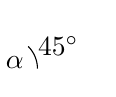
\begin{tikzpicture}[>=stealth]
\tkzDefPoints{0/0/A, 4/0/B, 1.5/1.5/D, 5.5/1.5/C}
\tkzDrawPolygon[thick](A,B,C,D)
\draw(.4,0) arc (0:45:.4)node[right]{$45^{\circ}$};
\tkzLabelAngles[pos=.4](C,B,A){$\alpha$}
\tkzLabelPoints[above](C,D)
\tkzLabelPoints[below](A,B)
\end{tikzpicture}
\captionof{figure}{}
\end{minipage}

平面在空间的位置有各种可能，可以是水平的，也可以是竖直的，或倾斜的.

当平面是水平放置的时候，通常把平行四边形的锐角画成$45^{\circ}$，横边的长度画成邻边的两倍（图1.1）．

当一个空间图形是由若干个平面组成时，为了增强立体感，对于那些被遮部分的线段画成虚线，或者不画（图1.2）．

为了表示平面，我们常把希腊字母$\alpha$、$\beta$、$\gamma$等写在代表平面的平行四边形的一个角上，如平面$\alpha$，平面$\beta$、平面$\gamma$；也可以用代表平面的平行四边形的四个顶点、或者相对的两个顶点的大写英文字母作为这个平面的名称，如图1.1中的平面$\alpha$，平面$ABCD$，平面$AC$或者平面$BD$都表示了同一平面.

在立体几何里，对于点和直线仍然采用平面几何中常用的表示方法：用一个大写字母$A,B,C,\ldots$表示点，用一个小写字母，如$a,b,c,\ldots$或两个大写字母如$AB,BC,\ldots$表示直线.

\begin{figure}[htp]
    \centering
\begin{tikzpicture}[thick]
    \begin{scope}
\tkzDefPoints{0/0/A', 2/0/A, 3/0/A'', .8/1.2/B', 1/1.6/C}
\tkzDefPointBy[translation= from A' to B'](A) \tkzGetPoint{B}
\tkzDefPointBy[translation= from A' to B'](A'') \tkzGetPoint{B''}
\tkzDefPointBy[translation= from A' to B'](A'') \tkzGetPoint{B''}
\tkzDefPointBy[translation= from A to B](C) \tkzGetPoint{C'}
\tkzDrawSegments(A',A'' A',B' A,B A'',B'' B,B'' A,C C,C' C',B)
\tkzDefPointWith[linear, K=1.3](C,A) \tkzGetPoint{E}
\tkzDefPointBy[translation= from A to B](E) \tkzGetPoint{E'}
\tkzInterLL(B',B)(A,C) \tkzGetPoint{tmp1}
\tkzInterLL(A',A)(E,E') \tkzGetPoint{tmp2}
\tkzDrawSegments[dashed](tmp1,B E,tmp2 E',B E',tmp2)
\tkzDrawSegments(A,E B',tmp1 tmp2,E)
\tkzLabelPoints[above right](B)
\tkzLabelPoints[below left](A)
\tkzLabelAngles[pos=.4](A,A',B'){$\alpha$}
\tkzLabelAngles[pos=.4](A,C,C'){$\beta$}
\node at (2,-1){甲};
    \end{scope}
    \begin{scope}[xshift=5cm]
\tkzDefPoints{0/0/A', 1/1/A, 4.5/1/B, 1/2.5/A'', 4.5/.25/E, .5/.25/E'}
\tkzDefPointBy[translation= from A to B](A') \tkzGetPoint{B'}
\tkzDefPointBy[translation= from A to B](A'') \tkzGetPoint{B''}
\tkzDrawPolygon(A,B,B',A')
\tkzDrawPolygon(A,B,B'',A'')
\tkzInterLL(E,E')(B,B')\tkzGetPoint{tmp1}
\tkzDrawSegments(tmp1,E E,B)
\tkzLabelPoints[ right](B)
\tkzLabelPoints[ left](A)
\tkzDefPointWith[linear, K=1.8](B',B) \tkzGetPoint{F}
\tkzDefPointBy[translation= from B to A](F) \tkzGetPoint{F'}
\tkzInterLL(F,F')(B,B'')\tkzGetPoint{tmp2}
\tkzDrawSegments(tmp2,F F,B)
\node at (2.5,-1){乙};
\tkzLabelAngles[pos=.4](B',A',A){$\alpha$}
\tkzLabelAngles[pos=.4](A,A'',B''){$\beta$}
    \end{scope}
\end{tikzpicture}
    \caption{}
\end{figure}

\subsection*{1.1 练习}

\begin{enumerate}
    \item 能不能说一条直线长3米，宽0.01米？为什么？
    \item 能不能说一个平面长3米，宽2米？为什么？
    \item 观察甲、乙两个图形，用模型来说明它们的区别。
\begin{center}
\begin{tikzpicture}[thick, scale=.9]
\begin{scope}
\tkzDefPoints{-1/.8/A, 0/0/A1, 1/.8/A2, -1/3/A', 2/0/A4, 3/0.8/A5, 4/0/A6}
\foreach \x in {1,2,4,5,6}
{
    \tkzDefPointBy[translation= from A to A'](A\x) \tkzGetPoint{A\x'}
}
\tkzDrawPolygon(A,A1,A2,A2',A1',A')
\tkzDrawPolygon(A4,A5,A6,A6',A5',A4')
\tkzDrawSegments(A1,A1' A5,A5')
\draw(-1.2,2)--(-.5,2);
\draw(.5,2)--(1.2,2);
\tkzDrawPoint(-.5,2)
\tkzDrawPoint(.5,2)
\draw(1.5,2)--(2,2);
\draw(2.5,2)--(3.5,2);
\draw(4,2)--(4.5,2);
\tkzDrawPoint(2.5,2)
\tkzDrawPoint(3.5,2)
\node at (0,-.5){甲};
\node at (3,-.5){乙};
\node at (1.5,-1){第3题};

\end{scope}
\begin{scope}[xshift=6cm]
\tkzDefPoints{0/0/A, 2/0/B, 1.5/.5/C, 0/2.5/A_1}
\foreach \x in {B,C}
{
    \tkzDefPointBy[translation= from A to A_1](\x) \tkzGetPoint{\x_1}
}
\tkzDrawPolygon(A_1,B_1,C_1)
\tkzDrawSegments[dashed](A,C B,C C,C_1)
\tkzDrawSegments(A_1,A A,B B,B_1)
\tkzLabelPoints[left](A_1,A)
\tkzLabelPoints[right](B_1,B)
\tkzLabelPoints[above left](C_1,C)

\tkzDefPoints{3/0.5/C, 5/.5/B, 3.5/0/A, 3.5/2.5/A_1}
\foreach \x in {B,C}
{
    \tkzDefPointBy[translation= from A to A_1](\x) \tkzGetPoint{\x_1}
}
\tkzDrawPolygon(B_1,C_1,C,A,B)
\tkzDrawSegments[dashed](C,B)
\tkzDrawSegments(A_1,C_1 A_1,B_1 A,A_1)
\tkzLabelPoints[left](C_1,C)
\tkzLabelPoints[right](B_1,B)
\tkzLabelPoints[below right](A_1)
\tkzLabelPoints[below ](A)
\node at (1,-.5){甲};
\node at (4,-.5){乙};
\node at (2.5,-1){第4题};
\end{scope}

\end{tikzpicture}
\end{center}
    
\noindent
\begin{minipage}{.5\textwidth}
    \item  观察甲、乙两个图形，写出它们由哪些面围成？
    \item 右图是尚未画好的图形. 请你根据下面的要求，把被遮住的部分改为虚线.
\begin{enumerate}[(1)]
\item $AB$没有被平面$\alpha$遮挡；
\item $AB$被平面$\alpha$遮挡．
\end{enumerate}
\end{minipage}
\hfill
\begin{minipage}{.45\textwidth}
\centering
\begin{tikzpicture}[>=stealth]
\tkzDefPoints{0/0/B1, 1.5/.5/B, 3/1/B2, 1.5/3.5/B', .5/1/A, 2.5/0/A'}

\tkzDefPointBy[translation= from B to B'](B1) \tkzGetPoint{B_1}
\tkzDefPointBy[translation= from B to B'](A) \tkzGetPoint{A_1}
\tkzDefPointBy[translation= from B to B'](A') \tkzGetPoint{A_2}
\tkzDefPointBy[translation= from B to B'](B2) \tkzGetPoint{B3}

\tkzDrawPolygon(B1,B_1,B3,B2)
\tkzDrawPolygon(A,A_1,A_2,A')
\tkzDrawSegments(B,B')
\tkzLabelPoints[below](A,B)
\tkzLabelAngle[pos=.4](B,B1,B_1){$\alpha$}
\tkzLabelAngle[pos=.4](A_2,A',B){$\beta$}
\node at (1.5,-.5){第5题};
\end{tikzpicture}
\end{minipage}
\end{enumerate}

\section{平面的基本性质}
在生产和生活中，人们经过长期的观察和实践，总结出关于平面的三条基本性质，我们把它们作为公理，这些公理和我们在平面几何里已经学过的几个公理一起，构成了进一步推理的基础.

\begin{thm}
    {公理1}如果一条直线上的两点在一个平面内，那么这条直线上所有的点都在这个平面内.
\end{thm}

这时我们说“直线在平面内”，或者“平面经过直线”. 在这种情况下，直线上所有的点都在这个平面内，平面外的
任何一点都不在这条直线上.

这一公理描述了平面的平和无限延展的性质. 用直线的“直”来刻画平面的“平”，用直线的无限延伸刻画了平面的无限延展性.

公理1告诉我们，要判断一条直线在一个平面内，只需证明其上的两个点在这个平面内就可以了.

如图1.3，点$A$在直线$a$上，记作“$A\in a$”；点$C$在直线$a$外，记作“$C\notin a$”；点$A$在平面$\alpha$内，记作“$A\in\alpha$”；点$A$在平面$\alpha$外，记作“$A\notin \alpha$”；直线$a$在平面$\alpha$内，记作“$a\subset \alpha$”
.

这样，公理1用符号表示就是：

\begin{thm}{}
 已知点$A\in a$，点$B\in a$, 且$A\in \alpha$, $B\in\alpha$，则$a\subset\alpha$. 即已知平面$\alpha$，点$A\in a$点$B\in a$，且$A\in\alpha$, $B\in\alpha$，则对任意的点$P\in a$, 有$P\in \alpha$.   
\end{thm}


\noindent
\begin{minipage}{.45\textwidth}
\centering
\begin{tikzpicture}[>=stealth]
\tkzDefPoints{0/0/a, 4/0/b, 1.5/1.5/d, 5.5/1.5/c, 1.5/1/e, 4/.5/f}
\tkzDrawPolygon(a,b,c,d)
\tkzLabelAngle[pos=.4](b,a,d){$\alpha$}
\draw[very thick](e)--(f);
\tkzDefPointWith[K=.2, linear](e,f) \tkzGetPoint{A}
\tkzDefPointWith[K=.6, linear](e,f) \tkzGetPoint{B}
\tkzLabelPoints[below](A,B)
\tkzDrawPoints(A,B)
\end{tikzpicture}
\captionof{figure}{}
\end{minipage}
\hfill
\begin{minipage}{.45\textwidth}
\centering
\begin{tikzpicture}[>=stealth]
\tkzDefPoints{0/0/A', 2.5/0/A, 4/0/A'', 1.2/1.5/B', 1.6/1.7/C}
\tkzDefPointBy[translation= from A' to B'](A) \tkzGetPoint{B}
\tkzDefPointBy[translation= from A' to B'](A'') \tkzGetPoint{B''}
\tkzDefPointBy[translation= from A' to B'](A'') \tkzGetPoint{B''}
\tkzDefPointBy[translation= from A to B](C) \tkzGetPoint{C'}
\tkzDrawSegments(A',A'' A',B' A'',B'' B,B'' A,C C,C' C',B)
\tkzDefPointWith[linear, K=1.3](C,A) \tkzGetPoint{E}
\tkzDefPointBy[translation= from A to B](E) \tkzGetPoint{E'}
\tkzInterLL(B',B)(A,C) \tkzGetPoint{tmp1}
\tkzInterLL(A',A)(E,E') \tkzGetPoint{tmp2}
\tkzDrawSegments[dashed](tmp1,B)
\tkzDrawSegments(A,E B',tmp1 tmp2,E)

\tkzLabelAngles[pos=.4](A,A',B'){$\alpha$}
\tkzLabelAngles[pos=.4](C,C',B){$\beta$}

\tkzDrawSegments[very thick](A,B)
\tkzDefPointWith[K=.3, linear](A,B) \tkzGetPoint{P}
\tkzLabelPoints[above left](P)
\tkzDrawPoints(P)
\node at (3.25,1.25){$a$};
\end{tikzpicture}
\captionof{figure}{}
\end{minipage}

\begin{thm}
   {公理2} 如果两个平面有一个公共点，那么它们有且只有一条通过这个点的公共直线. 
\end{thm}

两个平面\footnote{今后凡说到两个平面，两条直线或两个点，如无特殊说明，均分别指两个不同的平面、直线和点.}有一条公共直线，我们就说这\textbf{两个平面相交}，它们的公共直线叫做两个平面的\textbf{交线}．如图1.4，平面$\alpha$与平面$\beta$相交，交线为$a$，说成“平面$\alpha$与$\beta$相交于直线$a$”，记作“$\alpha\cap\beta=a$”. 画两个平面相交，就要画出它们的交线.

公理2告诉我们：如果两个平面有一个公共点，那么这两个平面就一定相交，且其交线一定过这个公共点. 这就是说，如果两个平面有一个公共点，那么它们必定还有另外的公共点. 这就给我们提供了判断和论证两个平面是否相交，以及一点是否在两个平面交线上的依据. 即若$\alpha\cap \beta=\ell$，且$A\in\alpha$, $A\in\beta$，则$A\in\ell$.

\begin{thm}
  {公理3} 经过不在同一条直线上的三点，有且只有一个平面（图1.5）．  
\end{thm}


\noindent
\begin{minipage}{.45\textwidth}\CTEXindent
    例如，一扇门用两个合页和一把锁就可以固定了.

    过$A$、$B$、$C$三点的平面又可记作“平面$ABC$”.

    根据上述公理，可以得出下面的推论：
\end{minipage}
\hfill
\begin{minipage}{.5\textwidth}
\centering
\begin{tikzpicture}[>=stealth, scale=1.5]
\tkzDefPoints{0/0/A1, 3/0/B1, 1/1.5/D1, 4/1.5/C1}
\tkzDrawPolygon[thick](A1,B1,C1,D1)
\tkzLabelAngles[pos=.4](B1,A1,D1){$\alpha$}

\tkzDefPoints{1/.5/A, 2/1.1/B, 2.5/.4/C}
\tkzLabelPoints[above](A,B,C)
\tkzDrawPoints(A,B,C)
\end{tikzpicture}
\captionof{figure}{}
\end{minipage}

\begin{thm}
    {推论1} 经过一条直线和这条直线外的一点，有且只有一个平面（图1.6甲）．
\end{thm}

\begin{figure}[htp]
    \centering
\begin{tikzpicture}[scale=1]
\begin{scope}
\tkzDefPoints{0/0/A1, 3/0/B1, 1/1.5/D1, 4/1.5/C1}
\tkzDrawPolygon[](A1,B1,C1,D1)
\tkzLabelAngle[pos=.4](B1,A1,D1){$\alpha$}
\node at (1.5,-.5){甲};

\draw[ thick](.7,.25)--(3,.25);
\tkzDefPoints{1.15/0.25/B, 2.5/0.25/C, 2.2/1.1/A}
\tkzLabelPoints[above](B,C)
\tkzLabelPoints[right](A)
\tkzDrawPoints(A,B,C)

\end{scope}
\begin{scope}[xshift=4cm]
    \tkzDefPoints{0/0/A1, 3/0/B1, 1/1.5/D1, 4/1.5/C1}
\tkzLabelAngle[pos=.4](B1,A1,D1){$\alpha$}
\tkzDrawPolygon[](A1,B1,C1,D1)
    \node at (1.5,-.5){乙};
\tkzDefPoints{1/1.2/A, 3/.25/B, .8/.2/C, 3.4/1.3/D}
\tkzDrawSegments[very thick](A,B C,D)
\node at (A)[right=.2]{$b$};
\node at (C)[above]{$a$};
\end{scope}
\begin{scope}[xshift=8cm]
\tkzDefPoints{0/0/A1, 3/0/B1, 1/1.5/D1, 4/1.5/C1}
\tkzLabelAngle[pos=.4](B1,A1,D1){$\alpha$}
\tkzDrawPolygon[](A1,B1,C1,D1)
\node at (1.5,-.5){丙};
\tkzDefPoints{1/.2/A, 3/.5/B, 1/.8/C, 3/1.1/D}
\tkzDrawSegments[very thick](A,B C,D)
\node at (2,.5){$a$};
\node at (2,1.1){$b$};
\end{scope}

\end{tikzpicture}
    \caption{}
\end{figure}

\begin{thm}
    {推论2} 经过两条相交直线，有且只有一个平面（图1.6乙）.
\end{thm}


\begin{thm}
    {推论3} 经过两条平行直线，有且只有一个平面（图1.6丙）.
\end{thm}


“有且只有一个平面”也可以说是“确定一个平面。”


下面我们证明推论1．

已知：直线$a$及点$A$，且$A\notin a$.

求证：过直线$a$和点$A$有且只有一个平面.

\begin{analyze}
根据题意要证明的结论是下述两个命题：
\begin{enumerate}[(1)]
\item 过直线$a$和点$A$有一个平面（即存在着一个平面，直线$a$和点$A$都在这个平面内）.
\item 过直线$a$和点$A$只能有一个平面（即直线$a$和点$A$不可能同时在两个平面内）.
\end{enumerate}
\end{analyze}

证明的依据是已学过的公理，尤其是公理3和这里要证的结论是相同的，只是条件不同；这里给的条件是一条直线$a$和直线$a$外的一点$A$，而公理3是“不在同一直线上的三点”．我们只要在直线$a$上任取两点$B,C$，它们和点$A$就不共线，这正是公理3的已知条件所要求的．所以对第一个命题我们可以证明如下：

\begin{proof}
(1) 在$a$上任取两点$B$、$C$，由$A\notin a$知，$A$、$B$、$C$三点不共线，经过$A$、$B$、$C$三点可以有一个平面$\alpha$（公理3）．（图1.6甲）

$\because\quad B,C\in \alpha$

$\therefore\quad a\subset \alpha$（公理1），

$\therefore\quad $过$a$及$A$存在一个平面.
\end{proof}

\begin{analyze}
    欲证第二个命题，可以用反证法．反证法一般有四个步骤：
\begin{enumerate}
    \item 作一个和求证相反的假设；
    \item 用正确的推理导出矛盾；
    \item 否定我们作的那个假设；
    \item 肯定所要证明的结论.
\end{enumerate}
\end{analyze}

\begin{proof}
    （2）假设过$a$及$A$还有一个平面$\beta$，则$\beta$经过不共线的三点$A$、$B$、$C$，

$\therefore\quad$    经过$A$、$B$、$C$三点有两个平面$\alpha$和$\beta$，这与公理3矛盾，即知假设不成立，

$\therefore\quad $过$a$及$A$的平面只有一个，
于是，点$A$和直线$a$确定一个平面.
\end{proof}

\begin{note}
    上述两个命题的证明是不能互相代替的．（1）的证明所解决的问题是命题1，即存在着满足条件的平面：其着眼点是“存在”，并没有说不存在第二个平面．而（2）的证明只解决满足条件的平面不可能有两个，其着眼点是“不能有两个”，并没有说一定有平面．（1）（2）两个命题都被证明后，才能保证原题被完全证明了.
\end{note}

\begin{example}
    求证两两相交且不过同一点的三条直线必在同一平面内（$n$条直线两两相交就是每两条直线都相交）

已知：直线$\ell_1,\ell_2,\ell_3$, $\ell_1\cap \ell_2=A$\footnote{直线$a$和直线$b$相交于点$A$，我们规定记作$a\cap b=A$}, $\ell_2\cap \ell_3=B$, $\ell_3\cap \ell_1=C$.（图1.7）

求证：$\ell_1,\ell_2,\ell_3$共面.
\end{example}

\begin{analyze}
    证明$\ell_1,\ell_2,\ell_3$共
面，就是要找一个平面，使得三条直线$\ell_1,\ell_2,\ell_3$都在这个平面内. 关键是如何找到这个平面，也就是说如何确定这个平面.我们知道，确定平面有四种方法：

\noindent
\begin{minipage}{.53\textwidth}\CTEXindent
\begin{enumerate}
    \item 根据公理3，用不在同一直线上的三点；
    \item 根据推论1，用一条直线和这直线外的一个点；
    \item 根据推论2，用两条相交直线；
    \item 根据推论3，用两条平行直线.
\end{enumerate}
\end{minipage}
\hfill
\begin{minipage}{.45\textwidth}
\centering
\begin{tikzpicture}[scale=1.3]
    \tkzDefPoints{0/0/A1, 3/0/B1, 1/1.5/D1, 4/1.5/C1}
\tkzLabelAngle[pos=.4](B1,A1,D1){$\alpha$}
\tkzDrawPolygon[](A1,B1,C1,D1)
\tkzDefPoints{1/.5/B, 2.5/.35/C, 2/1.2/A}
\tkzDrawLines[add=.3 and .2](A,C B,C A,B)
\tkzLabelPoints[below](B,C)
\tkzLabelPoints[right](A)
\tkzDrawPoints(A,B,C)
\node at (1.7,1.3){$\ell_1$};
\node at (2.5,1.3){$\ell_2$};
\node at (2.9,.5){$\ell_3$};

\end{tikzpicture}
\captionof{figure}{}
\end{minipage}


具体证明时用哪种方法，就要看题目的已知条件中含有上述四条中的哪一条.

在本题中，已知的是三条直线，它们两两相交且不共点，即每两条直线都相交且三条直线不过同一点，我们可以选择哪一种方法来确定平面呢？

我们可以选取$A$，$B$，$C$三点，因为它们不共线，所以可以确定一个平面；也可以选择一条直线和这直线外的一点，例如$\ell_1$和点$B$；还可以选择两条相交直线例如$\ell_1$和$\ell_2$都可以确定平面，当确定平面以后再证明我们确定平面时未用到的直线也在这个面内，我们的证明就完成了.
\end{analyze}

\begin{proof}
\textbf{证法一：} $\because\quad \ell_1\cap \ell_2=A,\quad  \ell_2\cap \ell_3=B,\quad  \ell_3\cap\ell_1=C$

$\therefore\quad A,B,C$三点不共线（否则，$\ell_1,\ell_2,\ell_3$为同一直线，与题设矛盾）

$\therefore\quad A,B,C$三点确定一个平面设为$\alpha$（公理3）．

$\because\quad A\in \ell_2,\quad  B\in\ell_2$,

$\therefore\quad \ell_2\subset \alpha$（公理1）．

同理可证$\ell_1\subset\alpha,\quad  \ell_3\subset\alpha$,

$\therefore\quad \ell_1,\ell_2,\ell_3$共面．

\textbf{证法二：}$\because\quad B\notin \ell_1$，

$\therefore\quad \ell_1$和点$B$确定一个平面设为$\alpha$（推论1）

$\because\quad A\in \ell_1,\quad  \ell_1\subset\alpha$

$\therefore\quad A\in\alpha$.

$\because\quad A=\ell_1\cap \ell_2$

$\therefore\quad A\in \ell_2$

$\because\quad B=\ell_2\cap \ell_3$

$\therefore\quad B\in \ell_2$. 而$A\in\alpha,\quad  B\in\alpha$,

$\therefore\quad \ell_2\subset\alpha$（公理1），同理$\ell_3\subset\alpha$,

$\therefore\quad \ell_1,\ell_2,\ell_3$共面．

\textbf{证法三：}由已知$\ell_1\cap \ell_2=A$,

$\therefore\quad \ell_1$和$\ell_2$确定一个平面设为$\alpha$（推论2）

$\because\quad B\in \ell_2$,

$\therefore\quad B\in\alpha,\quad  C\in \ell_1$,

$\therefore\quad C\in\alpha$

$\because\quad B=\ell_2\cap \ell_3$,

$\therefore\quad B\in\ell_3$

$\because\quad C=\ell_1\cap \ell_3$,

$\therefore\quad C\in\ell_3$.

$\therefore\quad \ell_3\subset\alpha$（公理1），

$\therefore\quad \ell_1,\ell_2,\ell_3$都在$\alpha$内．
即$\ell_1,\ell_2,\ell_3$共面．
\end{proof}

\begin{remark}
    上述三种证法的共同点是：先利用已知的某些条件确定一个平面；然后再证明未用到的直线在这个平面内. 这是证明几条直线共面的一般思路.
\end{remark}

\subsection*{1.2 练习}
\begin{enumerate}
\item 用符号表示下列语句：
\begin{enumerate}[(1)]
\item 点$A$在平面$\alpha$内，但在平面$\beta$外；
\item 直线$a$经过平面$\alpha$外的一点$M$；
\item 直线$a$和直线$b$相交于平面$\alpha$内的一点$M$；
\item 直线$a$经过平面$\alpha$内的两点$M$和$N$．
\end{enumerate}

\item 读出下列符号并画图：
\begin{multicols}{2}
\begin{enumerate}[(1)]
    \item $A\in\alpha,\quad B\in\alpha,\quad  C\in AB$;
    \item $A\in\alpha,\quad a\not\subset\alpha,\quad A\in a$;
    \item $a\cap \alpha=A,\quad b\cap \alpha=A$;
    \item $a\cap b=A,\quad a\subset\alpha,\quad b\subset \alpha$;
    \item $\alpha\cap \beta =\emptyset,\quad a\subset\alpha,\quad b\subset\beta$.
\end{enumerate}    
\end{multicols}


\item 用文字语言叙述下列各命题，再判断它们是否正确，并说明理由.
\begin{enumerate}[(1)]
    \item 当$A\in\alpha$, $B\notin \alpha$时，直线$AB\subset\alpha$.
    \item $\begin{cases}
        A\in\alpha\\B\in\alpha\\C\in AB
    \end{cases}\Rightarrow\quad C\in \alpha$
\end{enumerate}   
\end{enumerate}

\section{水平放置的平面图形的直观图的画法}
为了学习、研究和应用的需要，常把空间图形画在纸上或黑板上，这就是用平面图形来表示空间图形. 例如，图1.8画的是一个正方体，图1.9画的是一个圆柱体．容易发现，这些画出的图形都不是空间图形的真实形状，正方体的各个面本来都是正方形，而在图1.8中，有一些面就画成了平行四边形；圆柱的底面本来是圆，在图1.9中却画成了椭圆．虽然这些平面图形不同于原来的空间图形，但是，看起来都有较强的立体感，近似地反映了人们直接观察的结果，这样的平面图形是一种空间图形的直观图.

\noindent
\begin{minipage}{.45\textwidth}
\centering
\begin{tikzpicture}[scale=2]
\tkzDefPoints{0/0/A, 1/0/B, 1.35/.35/C, .35/.35/D, 0/1/A_1}
\foreach \x in {B,C,D}
{
    \tkzDefPointBy[translation =  from A to A_1](\x) \tkzGetPoint{\x_1}
}  
\tkzDrawPolygon[](A,B,B_1,A_1)
\tkzDrawSegments(A_1,D_1 C_1,D_1 B_1,C_1 C,C_1 C,B)
\tkzDrawSegments[dashed](A,D C,D D,D_1)
\tkzLabelPoints[below](A,B)
\tkzLabelPoints[above](C_1,D_1)
\tkzLabelPoints[left](A_1,D)
\tkzLabelPoints[right](B_1,C)

\end{tikzpicture}
\captionof{figure}{}
\end{minipage}
\hfill
\begin{minipage}{.45\textwidth}
\centering
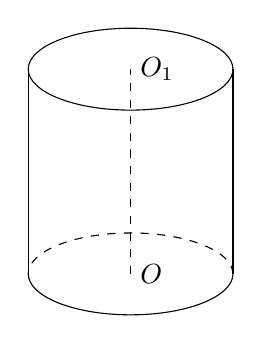
\begin{tikzpicture}[scale=1.3]
\draw(0,2) ellipse(1 and .4);
\draw[dashed](1,0)arc [start angle =0, end angle =180, x radius=1, y radius =.4];
\draw(1,0)arc [start angle =0, end angle =-180, x radius=1, y radius =.4];
\draw(-1,0)--(-1,2);
\draw(1,0)--(1,2);
\draw[dashed](0,0)node[right]{$O$}--(0,2)node[right]{$O_1$};
\end{tikzpicture}
\captionof{figure}{}
\end{minipage}

观察图1.8中的正方体和图1.9中的圆柱，可以看出两个底面变化非常明显，正方体的上、下底面画成了平行四边形，圆柱的上、底面由圆变成了椭圆，它们都是水平放置的平面图形.要画空间图形的直观图，首先要研究水平放置的平面
图形的直观图的画法. 下面举例说明一种常用的画法.

\begin{example}
画水平放置的正方形的直观图．
\end{example}

\begin{solution}
\textbf{画法：}
\begin{enumerate}[(1)]
    \item 在正方形$ABCD$所在的平面上，取$AB$所在的直线为$x$轴，取$AD$所在的直线为$y$轴，建立直角坐标系（图1.10）．设正方形$ABCD$的边长为$a$，则各顶点的坐标是$A(0,0)$, $B(a,0)$, $C(a,a)$, $D(0,a)$.
    
\noindent
\begin{minipage}{.6\textwidth}
\item 画对应的斜坐标系$x'O'y'$，使$\angle x'O'y'=45^{\circ}$， $O'y'$轴上的单位长取$O'x'$轴上单位长的一半. 在斜坐标系里，画$A$、$B$、$C$、$D$的对应点的方法是，横纵坐标与原来的保持不变，于是，得$A'(0,0)$, $B'(a,0)$, $C'(a,a)$, $D'(0,a)$.
\item 连结$A'B'$、$B'C'$、$C'D'$、$D'A'$，所得的四边形$A'B'C'D'$就是正方形$ABCD$的直观图.
\end{minipage}
\hfill
\begin{minipage}{.37\textwidth}
\centering
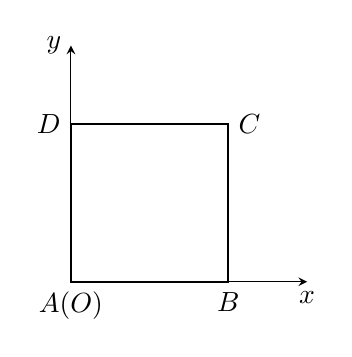
\begin{tikzpicture}[>=stealth]
\draw[->](0,0)node[below]{$A(O)$}--(3,0)node[below]{$x$};
\draw[->](0,0)--(0,3)node[left]{$y$};
\draw[thick](0,0)--(2,0)node[below]{$B$}--(2,2)node[right]{$C$}--(0,2)node[left]{$D$}--cycle;
\end{tikzpicture}
\captionof{figure}{}
\end{minipage}
\end{enumerate}
\end{solution}

\begin{rmk}
    图画好后，要擦去辅助线（图1.12），辅助线包括$x'$轴、$y'$轴以及为画图添加的线.
\end{rmk}

\noindent
\begin{minipage}{.45\textwidth}
    \centering
    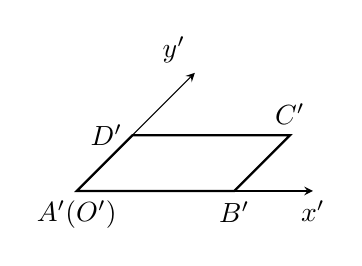
\begin{tikzpicture}[>=stealth]
    \draw[->](0,0)node[below]{$A'(O')$}--(3,0)node[below]{$x'$};
    \draw[->](0,0)--(1.5,1.5)node[above left]{$y'$};
\draw[thick](0,0)--(2,0)node[below]{$B'$}--(2+.707,.707)node[above]{$C'$}--(.707,.707)node[left]{$D'$}--cycle;
\end{tikzpicture}
\captionof{figure}{}
\end{minipage}
\hfill
\begin{minipage}{.45\textwidth}
\centering
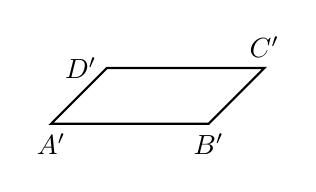
\begin{tikzpicture}[]
\draw[thick](0,0)node[below]{$A'$}--(2,0)node[below]{$B'$}--(2+.707,.707)node[above]{$C'$}--(.707,.707)node[left]{$D'$}--cycle;
\end{tikzpicture}
\captionof{figure}{}
\end{minipage}  

\begin{example}
     画水平放置的五边形$ABCDE$的直观图．
\end{example}

\begin{solution}
\textbf{画法：}
\begin{enumerate}[(1)]
\noindent
\begin{minipage}{.6\textwidth}
\item 以$AB$所在直线为$x$轴，以$AB$的垂直平分线
为$y$轴，建立直角坐标系，并画出$A$、$B$、$C$、$D$、$E$各点的坐标所对应的线段（图1.13）;
\item 画斜坐标系$x'O'y'$，使$\angle x'O'y'=45^{\circ}$；$O'y'$轴上的单位长取$O'x'$轴上单位长的一半.
\item 在$x'O'y'$中，画出$A$、$B$、$C$、$D$、$E$的对应点$A',B',C',D',E'$，使$A',B',C',D',E'$各点的横纵坐标分别等于$A,B,C,D,E$各点在$xOy$中的横纵坐标（图1.14）;
\end{minipage}
\hfill
\begin{minipage}{.38\textwidth}
\centering
\begin{tikzpicture}[>=stealth, scale=.9]
\draw[->](-2.5,0)--(2.5,0)node[below]{$x$};
\draw[->](0,-1)--(0,4)node[left]{$y$};
\tkzDefPoints{-1/0/A, 1/0/B, 1.62/1.9/C, -1.62/1.9/E, 0/3.1/D}
\tkzDrawPolygon[thick](A,B,C,D,E)
\draw[dashed](C)node[right]{$C$}--(1.62,0)node[below]{$C_1$};
\draw[dashed](E)node[left]{$E$}--(-1.62,0)node[below]{$E_1$};
\tkzLabelPoints[below](A,B)
\tkzLabelPoints[above right](D)
\tkzDefPoints{-1.62/0/E_1, 1.62/0/C_1, 2/0/C1}
\tkzMarkRightAngles[size=.15](E,E_1,A C,C_1,C1)
\end{tikzpicture}
\captionof{figure}{}
\end{minipage}

\item 连结$A'E'$、$E'D'$、$D'C'$、$C'B'$，则五边形$A'B'C'D'E'$就是正五边形$ABCDE$的直观图（图1.15）．
\end{enumerate}
\end{solution}

\noindent
\begin{minipage}{.45\textwidth}
\centering
\begin{tikzpicture}[>=stealth]
    \draw[->](-2.5,0)--(2.5,0)node[below]{$x'$};
    \draw[->](-.5,-.5)--(2,2)node[left]{$y'$};
    \tkzDefPoints{-1/0/A', 1/0/B', 1.62/0/C'_1, -1.62/0/E'_1, 0/0/O'}
\tkzDefPoints{-1.62+.67/.67/E', 1.62+.67/.67/C', 1.1/1.1/D'}
\tkzLabelPoints[below](A',B',C'_1,E'_1,O')
\tkzLabelPoints[above](E',D',C')
\tkzDrawPolygon[thick](A',B',C',D',E')
\tkzDrawSegments[dashed](E',E'_1 C',C'_1)
\end{tikzpicture}
\captionof{figure}{}
\end{minipage}
\hfill
\begin{minipage}{.45\textwidth}
\centering
\begin{tikzpicture}[]
    \tkzDefPoints{-1/0/A', 1/0/B', 1.62/0/C'_1, -1.62/0/E'_1}
\tkzDefPoints{-1.62+.67/.67/E', 1.62+.67/.67/C', 1.1/1.1/D'}
\tkzLabelPoints[below](A',B')
\tkzLabelPoints[above](E',D',C')
\tkzDrawPolygon[thick](A',B',C',D',E')
\end{tikzpicture}
\captionof{figure}{}
\end{minipage}

上面画直观图的方法叫做\textbf{斜二侧画法}，这样画的结果有三项不变.
\begin{enumerate}
\item 原图中的共线点，在直观图中仍是共线点，原图中的共点线，在直观图中仍是共点线.
\item 原图中的平行线，在直观图中仍是平行线．
\item 直观图中对应线段的比，仍等于原图中的平行线段（或共线线段）的比.
\end{enumerate}

因此，原图中的相等和相似的关系在直观图中仍然保持不变.


\subsection*{1.3 练习}
\begin{enumerate}
\item 画水平放置的正三角形的直观图. 
\item 画水平放置的等腰三角形、任意三角形的直观图．
\item 画水平放置的平行四边形、矩形的直观图。
\item 画水平放置的正六边形的直观图.
\end{enumerate}

\section*{习题一}
\begin{center}
    \bfseries A
\end{center}
\begin{enumerate}
    \item 下面的说法正确吗？为什么？
\begin{enumerate}[(1)]
 \item 线段$AB$在$\alpha$内，但直线$AB$不全在平面$\alpha$内。
\item 平面$\alpha$和平面$\beta$若有公共点，就不只一个。  
\end{enumerate}
    \item 改正下列作图中的错误．

    \item 改正下列表达式的错误：
\begin{enumerate}[(1)]
\item 直线$a$在平面$\alpha$内表示为$a\in\alpha$;
\item 平面$\alpha$与平面$\beta$相交表示为$\alpha\cap \beta$;
\item 直线$\ell$与平面$\alpha$相交表示为$\ell\cap\alpha$;
\item 直线$a$不在平面$\alpha$内表示为$a\notin \alpha$．
\end{enumerate}

\begin{figure}[htp]
    \centering
\begin{tikzpicture}[scale=.8]
\begin{scope}
\tkzDefPoints{0/0/A', 3/0/B', 3.75/1.5/C', .75/1.5/D'}
\tkzDrawPolygon[thick](A',B',C',D')
\node at (1.5,-1.5){(1)};
\tkzLabelAngle[pos=.5](B',A',D'){$\alpha$}
\tkzDefPoints{1.5/.8/A, 2.5/.8/B}
\tkzDrawLines[add=.7 and 1.5](A,B)
\tkzLabelPoints[below](A,B)
\tkzDrawPoints(A,B)
\node at (1.5,-2)[text width=4cm, align =center]{直线$AB$在$\alpha$内};


\end{scope}
\begin{scope}[xshift=5cm]
    \tkzDefPoints{0/0/A', 3/0/B', 3.75/1.5/C', .75/1.5/D'}
\tkzDrawPolygon[thick](A',B',C',D')
\tkzLabelAngle[pos=.5](B',A',D'){$\alpha$}
\node at (1.5,-1.5){(2)};
\tkzDefPoints{1.25/-1/A, 2.75/-.2/B, .8/2/D}
\tkzDefPointBy[translation = from A to B](D) \tkzGetPoint{C}
\tkzDrawPolygon[thick](A,B,C,D)
\tkzLabelAngle[pos=.5](D,C,B){$\beta$}
\node at (1.5,-2)[text width=4cm, align =center]{平面$\alpha$与$\beta$相交};

\end{scope}
\begin{scope}[xshift=10cm]
    \tkzDefPoints{0/0/A', 3/0/B', 3.75/1.5/C', .75/1.5/D'}
\tkzDrawPolygon[thick](A',B',C',D')
\tkzLabelAngle[pos=.5](B',A',D'){$\alpha$}
\node at (1.5,-1){(3)};
\draw(1,2.5)node[right]{$\ell$}--(2.5, -1);
\tkzDrawPoint(1.75, .75)
\node at (1.5,-2)[text width=6cm, align =center]{直线$\ell$与平面$\alpha$\\有一个公共点};
\end{scope}
\end{tikzpicture}
    \caption*{第2题}
\end{figure}

    \item 判断题：
\begin{enumerate}[(1)]
\item 空间三个点确定一个平面．\hfill(\qquad )
\item 空间四点任何三点不共线，则这四点不共面.\hfill(\qquad )
\item 空间四点共面而不共线，则四点中必有三点不共线.\hfill(\qquad )
\item 若三条直线两两相交，则这三条直线必共面.\hfill(\qquad )
\item 四边形不一定是平面图形。\hfill(\qquad )
\item 四个边都相等的四边形是菱形. \hfill(\qquad )
\item 如图第4题（7），$AB\parallel DE$，$AB\cap CD=A$．则过直线$AB$和点$D$的平面与过$AB$和$DE$的平面是同一个平面.\hfill(\qquad )

过$AB$和点$D$的平面与过$DE$和点$C$的平面是同一个平面.\hfill(\qquad )
\item 梯形一定是平面图形．\hfill(\qquad )
\end{enumerate}

\noindent
\begin{minipage}{.45\textwidth}
\centering
\begin{tikzpicture}[]
\tkzDefPoints{0/0/B, 1/2/A, 1.5/0/E, 2.5/2/D', 4/-0.5/C}
\tkzDrawSegments(A,B A,C D',E)  
\tkzInterLL(A,C)(D',E) \tkzGetPoint{D}
\tkzLabelPoints[below](B,E)
\tkzLabelPoints[above](A,C)
\tkzLabelPoints[right](D)
\tkzDrawPoints(A,D)


\end{tikzpicture}
\captionof*{figure}{第4题(7)}
\end{minipage}
\hfill
\begin{minipage}{.45\textwidth}
\centering
\begin{tikzpicture}[]
\tkzDefPoints{0/0/A, 2/0/B, 0/2/A_1, 2/2/B_1, .707/.707/D, 2/1/F}
\tkzDefPointBy[translation =  from A to D](B) \tkzGetPoint{C}  
\tkzDefPointBy[translation =  from A to D](B_1) \tkzGetPoint{C_1}  
\tkzDefPointBy[translation =  from A to D](A_1) \tkzGetPoint{D_1}  
\tkzDefPointBy[translation =  from A to D](F) \tkzGetPoint{E}  
\tkzDrawPolygon(A_1,B_1,B,A)
\tkzDrawSegments[dashed](A,D D,C D,D_1)
\tkzDrawSegments[](A_1,D_1 D_1,C_1 B_1,C_1 C,C_1 B,C)
\tkzLabelPoints[left](A,A_1,D,D_1,F)
\tkzLabelPoints[right](B,B_1,C,C_1,E)
\tkzDrawPoints(E,F)


\end{tikzpicture}
\captionof*{figure}{第5题}
\end{minipage}


\item 已知正方体$ABCD-A_1B_1C_1D_1$中，$E$、$F$分别是$C_1C$和$B_1B$的中点，画出
\begin{enumerate}[(1)]
 \item 直线$D_1E$与平面$ABCD$的交点；
\item 直线$C_1F$与平面$ABCD$的交点；
\item 直线$D_1F$与平面$ABCD$的交点；
\item 直线$A_1E$与平面$ABCD$的交点． 
\end{enumerate}

\noindent
\begin{minipage}{.45\textwidth}
\centering
\begin{tikzpicture}[]
\tkzDefPoints{0/0/B, 3/0/C, 1.35/.7/D, 1/2.5/A, 1.4/0/G}
\tkzDrawSegments[thick](B,D)
\tkzDrawPolygon[thick](A,B,C,D) 
\tkzLabelPoints[below](B,C,G)
\tkzLabelPoints[above](A)
\tkzDefPointWith[linear, K=.333](A,B) \tkzGetPoint{E}
\tkzDefPointWith[linear, K=.6](A,D) \tkzGetPoint{F}
\tkzLabelPoints[left](E)
\tkzLabelPoints[right](F)
\tkzLabelPoints[above right](D)
\tkzDrawPoints(E,F,G)
\end{tikzpicture}
\captionof*{figure}{第6题}
\end{minipage}
\hfill
\begin{minipage}{.45\textwidth}
\centering
\begin{tikzpicture}[]
\tkzDefPoints{0/0/A1, 3.5/0/B1, 1.25/1.5/D1}
\tkzDefPointBy[translation =  from A1 to D1](B1) \tkzGetPoint{C1}  
\tkzDrawPolygon[thick](A1,B1,C1,D1)
\tkzLabelAngle[pos=.4](B1,A1,D1){$\alpha$}
\tkzDefPoints{1/.5/Q, 2/.8/P, 3.75/1.21/R}
\tkzLabelPoints[below](P,Q,R)
\tkzDrawPoints(P,Q,R)
\tkzDefPoints{3/3.2/A}
\tkzDefPointWith[linear, K=.3](A,R) \tkzGetPoint{C} 
\tkzDrawSegments[thick](A,P A,R Q,C)
\tkzInterLL(C,Q)(A,P) \tkzGetPoint{B}
\tkzLabelPoints[left](B)
\tkzLabelPoints[right](C)
\tkzLabelPoints[above](A)


\end{tikzpicture}
\captionof*{figure}{第7题}
\end{minipage}


\noindent
\begin{minipage}{.57\textwidth}

\item 已知$A$点在平面$BCD$外，连结$AB$、$AD$. $E\in AB$, $AE=\frac{1}{3}AB$; $F\in AD$, $AF=FD$; $G\in BC$. 画出$CD$与平面$EFG$的交点$H$.
\item 已知$\triangle ABC$三边所在的直线分别交平面$\alpha$于$PQR$.

求证：$PQR$三点在同一直线上，
\item 证明两两相交但不过同一点的四条直线共面。
\item 画出图中水平放置的四边形$OABC$的直观图。
\end{minipage}
\hfill
\begin{minipage}{.4\textwidth}
\centering
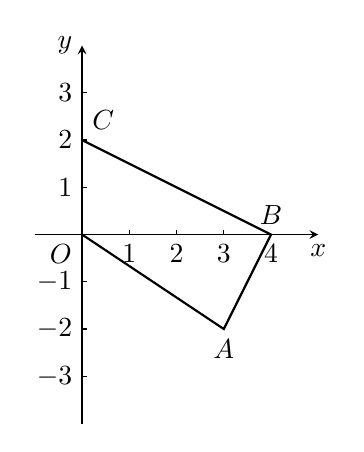
\begin{tikzpicture}[>=stealth, scale=.6]
\draw[->](-1,0)--(5,0)node[below]{$x$};
\draw[->](0,-4)--(0,4)node[left]{$y$};
\draw[thick](0,2)node[above right]{$C$}--(4,0)node[above]{$B$}--(3,-2)node[below]{$A$}--(0,0)node[below left]{$O$};
\foreach \x in {1,2,3}
{
    \draw(\x,0)node[below]{$\x$}--(\x,.1);
    \draw(0,-\x)node[left]{$-\x$}--(.1,-\x);
    \draw(0,\x)node[left]{$\x$}--(.1,\x);
}
\node at (4,0)[below]{$4$};

\end{tikzpicture}
\captionof*{figure}{第9题}
\end{minipage}
\end{enumerate}

\section*{二、空间两条直线}
\section{空间两条直线的位置关系}
在平面几何中我们知道，在同一平面内的两条直线的位置关系有两种：平行和相交.

空间的两条直线除了平行和相交以外，还有别的位置关系吗？观察正方体$ABCD-A_1B_1C_1D_1$（图1.16）．

棱$AB$和棱$DD_1$所在的直线会相交吗？是平行线吗？它们既不平行，又不相交，它们是不在同一平面内的直线. 

\begin{figure}[htp]
    \centering
    \begin{tikzpicture}[scale=2]
\tkzDefPoints{0/0/A, 1/0/B, 1.35/.35/C, .35/.35/D, 0/1/A_1}
\foreach \x in {B,C,D}
{
    \tkzDefPointBy[translation =  from A to A_1](\x) \tkzGetPoint{\x_1}
}  
\tkzDrawPolygon[](A,B,B_1,A_1)
\tkzDrawSegments(A_1,D_1 C_1,D_1 B_1,C_1 C,C_1 C,B)
\tkzDrawSegments[dashed](A,D C,D D,D_1)
\tkzLabelPoints[below](A,B)
\tkzLabelPoints[above](C_1,D_1)
\tkzLabelPoints[left](A_1,D)
\tkzLabelPoints[right](B_1,C)

\end{tikzpicture}
    \caption{}
\end{figure}

\begin{thm}
   {定义} 不可能在同一个平面内的两条直线，称为\textbf{异面直线}. 
\end{thm}

很明显，既不相交，也不平行（即不可能共面）的两条直线，就是异面直线.

这样，空间两条直线的位置关系有三种：
\begin{enumerate}
    \item 相交直线——在同一平面内，有且只有一个公共点;              
    \item 平行直线——在同一平面内，没有公共点；
    \item 异面直线——不同在任何一个平面内，没有公共点.
\end{enumerate}

\begin{figure}[htp]
    \centering
\begin{tikzpicture}
\begin{scope}
\tkzDefPoints{0/0/A, 2.5/0/B, 3/1/C, .5/1/D}
\tkzDrawPolygon[](A,B,C,D)
\tkzLabelAngles[pos=.4](B,A,D){$\alpha$}
\draw[thick](.75,.3)--node[above]{$a$}(2.3,.3);
\tkzDefPoints{2/2/A1, 3/-.5/A2}
\tkzDefPointWith[linear, K=.5](A1,A2) \tkzGetPoint{P}
\tkzInterLL(A1,A2)(B,C) \tkzGetPoint{Q}
\draw(A1)node[right]{$b$}--(P); \draw(A2)--(Q);
\tkzDrawPoints(P)

\end{scope}
\begin{scope}[xshift=4cm]
    \tkzDefPoints{0/0/A, 2.5/0/B, 3/1/C, .5/1/D, -.25/2/E}
    \tkzDefPointBy[translation = from D to E](C) \tkzGetPoint{F}
\tkzDrawPolygon[](C,D,E,F)
\tkzDrawPolygon[](A,B,C,D)
\tkzLabelAngles[pos=.4](B,A,D){$\alpha$}
\draw[thick](1.25,.25)--node[left]{$a$}(2.3,1);
\draw[thick](0.7,1.8)--node[right]{$b$}(1,1);
\tkzLabelAngles[pos=.5](D,E,F){$\beta$}


\end{scope}
\begin{scope}[xshift=8cm]
    \tkzDefPoints{0/0/A, 2.5/0/B, 3/1/C, .5/1/D}

\tkzDrawPolygon(A,B,C,D)
\tkzLabelAngles[pos=.4](B,A,D){$\alpha$}
\draw[thick](.75,.25)--node[above]{$a$}(2.5,.7);
\draw[thick](1,1.8)--node[above]{$b$}(2.6,1.8);

\end{scope}
\end{tikzpicture}
    \caption{}
\end{figure}


为了显示出异面直线不共面的特点，作图时，通常用一个或两个平面衬托，画成图1.17那样．

怎样判断两条直线是不是异
面直线呢？

\begin{thm}
    {定理} 平面内一点和平面外一点的连线，与平面内不经过该点的直线是异面直线.
\end{thm}

已知：$B\in \alpha$, $A\notin \alpha$, $a\subset\alpha$, $B\notin a$（图1.18），

求证：直线$AB$和$a$是异面直线.

\begin{analyze}
    要证明$AB$和$a$是异面直线，就是要证明它们不可能在同一平面内，可以采用反证法证明.
\end{analyze}

\begin{proof}
假设直线$AB$和$a$不是异面直线，则$AB$和$a$共面，设为$\beta$.

\noindent
\begin{minipage}{.61\textwidth}\CTEXindent
$\therefore\quad B\in\beta,\quad a\subset \beta$

$\because\quad B\in\alpha,\quad a\subset\alpha$，且$\beta\notin a$

$\therefore\quad \alpha$与$\beta$重合.

又$\because\quad A\in\beta$

$\therefore\quad A\in \alpha$，这与已知$A\notin\alpha$矛盾，

$\therefore\quad $假设不成立，即$AB$与$a$为异面直线. 
\end{minipage}
\hfill
\begin{minipage}{.34\textwidth}
\centering
\begin{tikzpicture}[scale=1.3]
    \tkzDefPoints{0/0/A1, 2.5/0/B1, 3/1/C1, .5/1/D1}
    \tkzDrawPolygon[](A1,B1,C1,D1)
    \tkzLabelAngles[pos=.4](B1,A1,D1){$\alpha$}
    \draw[thick](.75,.3)--node[above]{$a$}(2.3,.3);
    \tkzDefPoints{1.2/2/A, 2/-.5/A2}
    \tkzDefPointWith[linear, K=.5](A,A2) \tkzGetPoint{B}
    \tkzInterLL(A,A2)(A1,B1) \tkzGetPoint{Q}
    \draw(A)node[right]{$A$}--(B)node[right]{$B$}; \draw(A2)--(Q);
    \tkzDrawPoints(B)
\end{tikzpicture}
\captionof{figure}{}
\end{minipage}

\end{proof}

这样，判定空间两条直线是否异面直线，就有了两种方法，第一个方法是根据定义，用反证法能证明它们不可能是共面直线的，就是异面直线. 第二个方法是利用刚才证明的定理，可直接判定两条直线是不是异面直线.


\subsection*{1.4 练习}
\begin{enumerate}
\item 用1.4节所学的定理说明图1.17左边两个图的画法是正确的.
\item 找出日常生活中所遇到的异面直线的几个例子．
\item 两条平行直线没有公共点，能否说没有公共点的两条直线叫做平行直线呢？
\item 直线$a\subset$平面$\alpha$，直线$b\subset$平面$\beta$，$a$，$b$一定是异面直线吗？
\item 能否把异面直线的定义改为：“在空间没有公共点的直线？”为什么？
\item \begin{enumerate}[(1)]
    \item 怎样作一条直线，使之和已知的两条异面直线都相交？
    \item 与两条异面直线都相交的两条直线可能相交吗？画出图来。
    \item 与两条异面直线都相交的两条直线在什么情况下会是异面直线？请给予证明。
\end{enumerate}

\item 说出正方体中下列各对线段所在直线的位置关系：
\begin{multicols}{3}
\begin{enumerate}[(1)]
 \item $AB$和$CC_1$
\item $DD_1$和$CB_1$
\item $A_1C$和$BB_1$
\item $BD_1$和$DC$
\item $BD_1$和$A_1B_1$
\item $CD_1$和$DC_1$
\end{enumerate}
\end{multicols}

\noindent
\begin{minipage}{.45\textwidth}
    \centering
    \begin{tikzpicture}[scale=2]
\tkzDefPoints{0/0/A, 1/0/B, 1.35/.35/C, .35/.35/D, 0/1/A_1}
\foreach \x in {B,C,D}
{
    \tkzDefPointBy[translation =  from A to A_1](\x) \tkzGetPoint{\x_1}
}  
\tkzDrawPolygon[](A,B,B_1,A_1)
\tkzDrawSegments(A_1,D_1 C_1,D_1 B_1,C_1 C,C_1 C,B)
\tkzDrawSegments[dashed](A,D C,D D,D_1)
\tkzLabelPoints[below](A,B)
\tkzLabelPoints[above](C_1,D_1)
\tkzLabelPoints[left](A_1,D)
\tkzLabelPoints[right](B_1,C)

\end{tikzpicture}
\captionof*{figure}{第7题}

\end{minipage}
\hfill
\begin{minipage}{.45\textwidth}
\centering
\begin{tikzpicture}[]
\tkzDefPoints{0/0/B, 3/0/D, 1.5/2/A, 2/-.8/C}
\tkzDrawPolygon[thick](A,B,C,D)
\tkzDrawSegments(A,C)
\tkzDrawSegments[dashed](B,D)
\tkzLabelPoints[below](C)
\tkzLabelPoints[left](B)
\tkzLabelPoints[right](D)
\tkzLabelPoints[above](A)
\end{tikzpicture}
\captionof*{figure}{第8题}
\end{minipage}

\item 如图点$A$在平面$BCD$外，连结$AB$，$AC$，$AD$，在图中有
几对异面直线？能否有两条平行直线？
\end{enumerate}

\section{平行直线}
在平面几何里，我们在判定两直线平行时，有下述定理：“在同一个平面内，如果两条直线都和第三条直线平行，
那么这两条直线也互相平行.” 若三条直线不在同一平面内呢？上述论断同样成立. 我们把它作为公理.

\begin{thm}
    {公理4} 平行于同一直线的两条直线互相平行．
\end{thm}

\noindent
\begin{minipage}{.65\textwidth}\CTEXindent
    在正方体$ABCD-A_1B_1C_1D_1$中（图1.19）

    $\because\quad BC\parallel B_1C_1,\quad A_1D_1\parallel B_1C_1$
    
    $\therefore\quad BC\parallel A_1D_1$
    
    又$\because\quad BC=A_1D_1$
    
    $\therefore\quad A_1BCD_1$是平行四边形，
    
    $\therefore\quad A_1B\parallel CD_1$
\end{minipage}
\hfill
\begin{minipage}{.33\textwidth}
\centering
\begin{tikzpicture}[scale=2]
\tkzDefPoints{0/0/A, 1/0/B, 1.35/.35/C, .35/.35/D, 0/1/A_1}
\foreach \x in {B,C,D}
{
    \tkzDefPointBy[translation =  from A to A_1](\x) \tkzGetPoint{\x_1}
}  
\tkzDrawPolygon[](A,B,B_1,A_1)
\tkzDrawSegments(A_1,D_1 C_1,D_1 B_1,C_1 C,C_1 C,B A_1,B)
\tkzDrawSegments[dashed](A,D C,D D,D_1 C,D_1)
\tkzLabelPoints[below](A,B)
\tkzLabelPoints[above](C_1,D_1)
\tkzLabelPoints[left](A_1,D)
\tkzLabelPoints[right](B_1,C)


\end{tikzpicture}
\captionof{figure}{}
\end{minipage}



\begin{example}
    已知：四边形$ABCD$是空间四边形（四个顶点不共面的四边形），$E$、$H$分别是边$AB$、$AD$的中点，$F$、$G$分别是边$CB$、$CD$上的点，且$\frac{CF}{CB}=\frac{CG}{CD}=\frac{2}{3}$. 
    求证：\begin{enumerate}[(1)]
        \item 四边形$EFGH$是梯形．
        \item $EF$和$HG$的交点在直线$AC$上．
    \end{enumerate}
\end{example}

\begin{proof}
如图1.20，连结$BD$

\begin{enumerate}[(1)]
\noindent
\begin{minipage}{.6\textwidth}\CTEXindent

    \item $\because\quad EH$是$\triangle ABD$的中位线

$\therefore\quad EH\parallel BD,\quad EH=\frac{1}{2}BD$

又在$\triangle BCD$中，$\frac{CF}{CB}=\frac{CG}{CD}=\frac{2}{3}$,

$\therefore\quad FG\parallel BD,\quad FG=\frac{2}{3}BD$.

根据公理4，$EH\parallel FG$

又$\because\quad FG>EH$,

$\therefore\quad $四边形$EFGH$是梯形.
\end{minipage}
\hfill
\begin{minipage}{.38\textwidth}
\centering
\begin{tikzpicture}[scale=1.3]
\tkzDefPoints{0/0/B, 3/0/C, 1/0/F, 1.5/1/D, .9/2.5/A}
\tkzDrawPolygon[thick](A,B,C,D)

\tkzDefMidPoint(A,B) \tkzGetPoint{E}
\tkzDefMidPoint(A,D) \tkzGetPoint{H}
\tkzDefPointWith[linear, K=0.3333](D,C) \tkzGetPoint{G}
\tkzDrawPolygon[pattern=north east lines](E,F,G,H)
\tkzLabelPoints[below](B,F,C)
\tkzLabelPoints[above](A)
\tkzLabelPoints[above right](G,D)
\tkzLabelPoints[right](H)
\tkzLabelPoints[left](E)

\tkzInterLL(B,D)(E,F) \tkzGetPoint{tmp}
\tkzDrawSegments[thick](B,tmp)
\tkzDrawSegments[dashed](tmp,D)

\end{tikzpicture}
\captionof{figure}{}
\end{minipage}

\item $\because\quad EF\subset $平面$ABC$，$HG\subset$平面$ADC$．

设$EF\cap HG=P$，则$P$是平面$ABC$和平面$ADC$的公共点.

又$\because\quad $平面$ABC\cap $平面$ADC=AC$

$\therefore\quad P\in AC$（公理2）．
\end{enumerate}
\end{proof}

为了进一步研究异面直线，我们先证明下述定理（通常叫做\textbf{等角定理}）

\begin{thm}
 {定理} 如果一个角的两边和另一个角的两边分别平行并且方向相同，那么这两个角相等.   
\end{thm}

已知：$\angle AOB$和$\angle A_1O_1B_1$的边$OA\parallel O_1A_1$，$OB\parallel O_1B_1$，且方向相同（图1.21）．    

求证：$\angle AOB=\angle A_1O_1B_1$


\noindent
\begin{minipage}{.48\textwidth}
\centering
\begin{tikzpicture}[]
\tkzDefPoints{0/0/O, 3/0/B, 2/1.25/A, .5/2.25/O_1}
\foreach \x in {A,B}
{
    \tkzDefPointBy[translation = from O to O_1](\x) \tkzGetPoint{\x_1}
}
\draw(A_1)--(O_1)--(B_1);
\draw(A)--(O)--(B);
\tkzLabelPoints[left](O,O_1)
\tkzLabelPoints[right](A,B,A_1,B_1)
\end{tikzpicture}
\captionof{figure}{}
\end{minipage}
\hfill
\begin{minipage}{.48\textwidth}
\centering
\begin{tikzpicture}[]
\tkzDefPoints{-.5/0/a, 3/0/b, .3/1.5/d, -.2/2.25/a'}
\tkzDefPointBy[translation = from  a to d](b) \tkzGetPoint{c}
\foreach \x in {b,c,d}
{
    \tkzDefPointBy[translation = from a to a'](\x) \tkzGetPoint{\x'}
}
\tkzDrawPolygon[](a,b,c,d)
\tkzDrawPolygon[](a',b',c',d')

\tkzDefPoints{.8/.4/O, 2.5/.4/B, 2.5/1.1/A, 1.8/.4/D}
\tkzDefPointWith[linear, K=.85](O,A) \tkzGetPoint{C}

\foreach \x in {O,A,B,C,D}
{
    \tkzDefPointBy[translation = from a to a'](\x) \tkzGetPoint{\x_1}
}
\draw[thick](A)--(O)--(B);
\draw[thick](A_1)--(O_1)--(B_1);
\draw[thick](C_1)--(D_1);
\draw[thick](C)--(D);


\tkzLabelPoints[below](D,C)
\tkzLabelPoints[below left](D_1)
\tkzLabelPoints[above](C_1)
\tkzLabelPoints[right](B,B_1, A_1,A)
\tkzLabelPoints[left](O,O_1)

\tkzInterLL(a',b')(O,O_1) \tkzGetPoint{tmp1}
\tkzInterLL(a',b')(C,C_1) \tkzGetPoint{tmp2}
\tkzInterLL(a',b')(D,D_1) \tkzGetPoint{tmp3}

\tkzDrawSegments[dashed](O_1,tmp1 C_1,tmp2 D_1,tmp3)
\tkzDrawSegments(O,tmp1 C,tmp2 D,tmp3)

\tkzLabelAngle[pos=.4](b,a,d){$\alpha$};
\tkzLabelAngle[pos=.4](b',a',d'){$\beta$};

\end{tikzpicture}
\captionof{figure}{}
\end{minipage}





\begin{analyze}
当$\angle AOB$、$\angle A_1O_1B_1$共面时，平面几何中已经证明，需要研究的是证明两个角不共面的情况.

类比平面几何中证明两个角相等最常用的方法是利用全等图形或相似形，于是根据题设，可考虑构造全等三角形或
相似三角形，借助三角形的三边，证明两个对应角相等.
\end{analyze}

\begin{proof}
在$OA$、$OA_1$、$OB$、$OB_1$上分取截取$OC=O_1C_1$、$OD=O_1D_1$，连结$OO_1$、$CC_1$、$DD_1$、$CD$、$C_1D_1$（图1.22）。

$\because\quad OB\parallel O_1B_1,\quad OD=O_1D_1$,

$\therefore\quad OO_1D_1D$是平行四边形．

$\therefore\quad OO_1\paraeq DD_1$，同理$OO_1\paraeq CC_1$.

于是由公理4得$CC_1\parallel DD_1$，且$CC_1=DD_1$,

$\therefore\quad $四边形$CC_1D_1D$是平行四边形．

$\therefore\quad CD=C_1D_1$. 即知$\triangle COD\cong \triangle C_1O_1D_1$

$\therefore\quad \angle AOB=\angle A_1O_1B_1$.
\end{proof}

同学们可以进一步思考：把上述定理条件中的“并且方向相同”改换成（1）并且方向相反；（2）$OA$和$O_1A_1$的方向相同，$OB$和$O_1B_1$的方向相反，则$\angle AOB$和$\angle A_1O_1B_1$的关系如何？

由本定理容易得出下面的推论：

\begin{thm}
    {推论} 如果两条相交直线和另两条相交直线分别平行，那么这两组直线所组成的锐角（或直角）相等.
\end{thm}

\begin{rmk}
    平面几何里的定理，对于非平面图形，并不都是正确的.例如，”四个边相等的四边形是菱形”在平面几何里是正确的，但对非平面图形，它就不正确了，同时，即便是在非平面图形中也正确的平面几何里的定理（如本节的等角定理），仍然需要经过证明才能应用.
\end{rmk}

\subsection*{1.5 练习}
\begin{enumerate}
    \item 把一张长方形的纸对折两次，打开后如第1题图那样，
说明为什么这些折痕是互相平行的.
\item 如第2题图，$AA'$、$BB'$、$CC'$不共面，且$BB'\paraeq AA'$，$CC'\paraeq AA'$.

求证：$\triangle ABC\cong \triangle A'B'C'$.

\item 画两个相交平面，并在这两个平面内各画一条直线，使它们成为（1）平行直线；（2）相交直线；（3）异面直线。


\noindent
\begin{minipage}{.48\textwidth}
\centering
\begin{tikzpicture}[]
\tkzDefPoints{0/0/a, 1/-.5/b, 1.5/.1/c, 2.5/-.4/d, 3.5/.2/e, 0/2/a'}
\foreach \x in {b,c,d,e}
{
    \tkzDefPointBy[translation = from a to a'](\x) \tkzGetPoint{\x'}
}
\tkzDrawPolygon[](a,b,c,d,e,e',d',c',b',a')
\tkzDrawSegments(b,b' c,c' d,d')
\end{tikzpicture}
\captionof*{figure}{第1题}
\end{minipage}
\hfill
\begin{minipage}{.48\textwidth}
\centering
\begin{tikzpicture}[]
\tkzDefPoints{0/0/A, 1.5/0/B, 1/.8/C, 1.6/2.25/A'}

\tkzDrawPolygon[](A,B,C)
\foreach \x in {B,C}
{
    \tkzDefPointBy[translation = from A to A'](\x) \tkzGetPoint{\x'}
}
\foreach \x in {A,B,C}
{
    \draw(\x)--(\x');
}
\draw(A')--(C')--(B');
\draw[dashed](A')--(B');

\tkzLabelPoints[left](A,A')
\tkzLabelPoints[right](B,B',C,C')
\end{tikzpicture}
\captionof*{figure}{第2题}
\end{minipage}

\item 在一块长方体形木块的$A_1C_1$面上有一点$P$，过点$P$画一条直线和棱$CD$平行，说明应该怎样画。
\item 如图，在正方体中，$AE=A_1E_1$, $AF=A_1F_1$. 求证：$EF\paraeq E_1F_1$.

\noindent
\begin{minipage}{.48\textwidth}
\centering
\begin{tikzpicture}[]
\tkzDefPoints{0/0/A, 3/0/B, 3.8/.8/C, 0/1.5/A_1, 2/2/P}
\tkzDefPointBy[translation = from B to C](A) \tkzGetPoint{D}
\foreach \x in {B,C,D}
{
    \tkzDefPointBy[translation = from A to A_1](\x) \tkzGetPoint{\x_1}
}
\tkzDrawPolygon[thick](A_1,B_1,C_1,D_1)
  
\tkzDrawSegments[thick](A,A_1 B,B_1 C,C_1 A,B B,C)
\tkzDrawSegments[dashed](A,D D,D_1 C,D)
\tkzLabelPoints[left](A,A_1,D_1,D)
\tkzLabelPoints[right](B,B_1,C_1,C, P)
\tkzDrawPoints(P)


\end{tikzpicture}
\captionof*{figure}{第4题}
\end{minipage}
\hfill
\begin{minipage}{.48\textwidth}
\centering
\begin{tikzpicture}[]
\tkzDefPoints{0/0/A, 2/0/B, 2.7/.7/C, 0/2/A_1, 1.3/0/F}
\tkzDefPointBy[translation = from B to C](A) \tkzGetPoint{D}
\tkzDefMidPoint(A,D) \tkzGetPoint{E}

\foreach \x in {B,C,D,E,F}
{
    \tkzDefPointBy[translation = from A to A_1](\x) \tkzGetPoint{\x_1}
}
\tkzDrawPolygon[thick](A_1,B_1,C_1,D_1)
  
\tkzDrawSegments[thick](A,A_1 B,B_1 C,C_1 A,B B,C E_1,F_1)
\tkzDrawSegments[dashed](A,D D,D_1 C,D E,F)
\tkzLabelPoints[left](A,A_1)
\tkzLabelPoints[above](E_1,E)
\tkzLabelPoints[below](F,F_1)
  
\end{tikzpicture}
\captionof*{figure}{第5题}
\end{minipage}

\item 已知：$E$、$F$、$G$、$H$分别是空间四边形的四条边$AB$、$BC$、$CD$、$DA$的中点，求证：$EG$和$FH$相交且互相平分。
\item 已知：直线$a$和$b$是异面直线，直线$c\parallel a$，直线$b$与$c$不相交。求证：直线$b$、$c$是异面直线。
\end{enumerate}

\section{两条异面直线所成的角及它们的距离}
为了进一步研究两条异面直线之间的位置关系，我们引入“两条异面直线所成的角”和“两条异面直线间的距离”这样两个概念.

\begin{thm}
 {定义} 如果两条相交直线分别平行于两条异面直线，这两条相交直线所成的锐角（或直角）叫做这两条异面直线所成的角。   
\end{thm}

由等角定理易证：上述定义中，无论相交直线的交点在何处，两条异面直线相互位置一旦确定，它们所成的角就确定了，特别地，两条相交直线中可以有一条直线与两条异面直线中的一条重合.

例如，图1.23中，直线$D_1C_1$和直线$B_1B$是异面直线，

$\because\quad C_1C\parallel B_1B$

$\therefore\quad \angle D_1C_1C$就是异面直线$D_1C_1$与$B_1B$所成的角，即$D_1C_1$与$B_1B$成$90^{\circ}$角．

如果两条异面直线所成的角是直角，我们就说这两条异面直线互相垂直.


\noindent
\begin{minipage}{.45\textwidth}
\centering
\begin{tikzpicture}[]
\tkzDefPoints{0/0/A, 2/0/B, 2.7/.7/C, 0/2/A_1}
\tkzDefPointBy[translation = from B to C](A) \tkzGetPoint{D}
\foreach \x in {B,C,D}
{
    \tkzDefPointBy[translation = from A to A_1](\x) \tkzGetPoint{\x_1}
}
\tkzDrawPolygon[thick](A_1,B_1,C_1,D_1)
  
\tkzDrawSegments[thick](A,A_1 B,B_1 C,C_1 A,B B,C)
\tkzDrawSegments[dashed](A,D D,D_1 C,D)
\tkzLabelPoints[left](A,A_1,D,D_1)
\tkzLabelPoints[right](B_1,B, C,C_1)
  
\end{tikzpicture}
\captionof{figure}{}
\end{minipage}
\hfill
\begin{minipage}{.45\textwidth}
\centering
\begin{tikzpicture}[]
\tkzDefPoints{0/0/A, 2/0/B, 2.7/.7/C, 0/2/A_1}
\tkzDefPointBy[translation = from B to C](A) \tkzGetPoint{D}
\foreach \x in {B,C,D}
{
    \tkzDefPointBy[translation = from A to A_1](\x) \tkzGetPoint{\x_1}
}
\tkzDrawPolygon[thick](A_1,B_1,C_1,D_1)
  
\tkzDrawSegments[thick](A,A_1 B,B_1 C,C_1 A,B B,C B,C_1)
\tkzDrawSegments[dashed](A,D D,D_1 C,D)
\tkzLabelPoints[left](A,A_1,D,D_1)
\tkzLabelPoints[right](B_1,B, C,C_1)
\end{tikzpicture}
\captionof{figure}{}
\end{minipage}




\begin{example}
     如图1.24，在正方体$ABCD-A_1B_1C_1D_1$中：
\begin{enumerate}[(1)]
\item 有哪些棱所在的直线与直线$BC_1$成异面直线？求直线$BC_1$和它们所成角的大小；
\item 求直线$BC_1$和面对角线$CD_1$所成角的大小．
\end{enumerate}
\end{example}

\begin{solution}
\begin{enumerate}[(1)]
    \item 由图1.24易知，$AD\subset$平面$ABCD$，$C_1\notin$平面$ABCD$，$B\in$平面$ABCD$，$B\notin AD$，

$\therefore\quad    AD$和$BC_1$成异面直线．

同理：$A_1D_1$、$A_1A$、$D_1D$、$A_1B_1$、$CD$均与$BC_1$成异面直线.

$\because\quad BC\parallel AD$

$\therefore\quad \angle C_1BC$即为异面直线$AD$和$BC_1$所成的角.

而$BC=CC_1,\quad C_1C\bot BC$,

$\therefore\quad \angle C_1BC=45^{\circ}$，即异面直线$AD$和$BC_1$成$45^{\circ}$角．

同理$A_1D_1$、$A_1A$、$D_1D$、$A_1B_1$、$CD$和$BC_1$所成角均为$45^{\circ}$.

\item 连结$A_1B$、$A_1C_1$，则由$BC\paraeq AD$, $A_1D_1\paraeq AD$得四边形$BA_1D_1C$为平行四边形，

$\therefore\quad A_1B\parallel CD_1$

$\therefore\quad \angle A_1BC_1$即为异面直线$BC_1$和$CD_1$所成的角．

$\because\quad $正方体是六个面全等的正方形，

$\therefore\quad $面对角线$A_1B=BC_1=A_1C_1$，且长均为正方体棱长的$\sqrt{2}$倍.

$\therefore\quad \triangle A_1BC_1$为正三角形，$\angle A_1BC_1=60^{\circ}$

于是，异面直线$BC_1$和$CD_1$成$60^{\circ}$角．

\end{enumerate}
\end{solution}

图1.25中，正方体的棱$AA_1$和$B_1C_1$所在的直线是两条异面直线、直线$A_1B_1$和它们都垂直相交．

\begin{thm}
    {定义} 和两条异面直线都垂直相交的直线叫做\textbf{两条异面直线的公垂线}.
\end{thm}

为了确切地说明两条异面直线的相互位置，除了考虑它们所成的角的大小以外，还有一个如何表示它们离开得远近的问题．例如，在（图1.25）所示的长方体中，尽管$B_1D_1$和$BC$、$EF$、$GH$都成异面直线，并且它们与$B_1D_1$均成相等的角（$BC\parallel EF\parallel GH\parallel  B_1G_1$），但是，它们与$B_1D_1$离开的程度有远有近. 因此，我们还必须引入一个新的概念.

\begin{thm}
 {定义} 两条异面直线的公垂线在这两条异面直线间的线段的长度，叫做\textbf{两条异面直线的距离}。
  
\end{thm}
 
 图1.25中，线段$BB_1$的长度就是异面直线$A_1B_1$和$BC$的距离． 


\noindent
\begin{minipage}{.45\textwidth}
\centering
\begin{tikzpicture}[]
\tkzDefPoints{0/0/A, 3/0/B, 3.7/.7/C, 0/2/A_1}
\tkzDefPointBy[translation = from B to C](A) \tkzGetPoint{D}
\foreach \x in {B,C,D}
{
    \tkzDefPointBy[translation = from A to A_1](\x) \tkzGetPoint{\x_1}
}
\tkzDrawPolygon[thick](A_1,B_1,C_1,D_1)
  
\tkzDrawSegments[thick](A,A_1 B,B_1 C,C_1 A,B B,C B_1,D_1)
\tkzDrawSegments[dashed](A,D D,D_1 C,D)

\tkzDefPointWith[linear, K=0.33](B,B_1) \tkzGetPoint{E}
\tkzDefPointWith[linear, K=0.67](B,B_1) \tkzGetPoint{G}
\tkzDefPointWith[linear, K=0.33](C,C_1) \tkzGetPoint{F}
\tkzDefPointWith[linear, K=0.67](C,C_1) \tkzGetPoint{H}

\tkzLabelPoints[left](A,A_1,D,D_1, G,E)
\tkzLabelPoints[right](B_1,B, C,C_1,F,H)

\tkzDrawSegments[thick](E,F G,H)

\end{tikzpicture}
\captionof{figure}{}
\end{minipage}
\hfill
\begin{minipage}{.45\textwidth}
\centering
\begin{tikzpicture}[]
    \tkzDefPoints{0/0/A, 2/0/B, 2.7/.7/C, 0/2/A_1}
    \tkzDefPointBy[translation = from B to C](A) \tkzGetPoint{D}
    \foreach \x in {B,C,D}
    {
        \tkzDefPointBy[translation = from A to A_1](\x) \tkzGetPoint{\x_1}
    }
    \tkzDrawPolygon[thick](A_1,B_1,C_1,D_1)
      
    \tkzDrawSegments[thick](A,A_1 B,B_1 C,C_1 A,B B,C)
    \tkzDrawSegments[dashed](A,D D,D_1 C,D)

\tkzDefMidPoint(B,C) \tkzGetPoint{E}
\tkzDefMidPoint(B_1,C_1) \tkzGetPoint{E_1}
\draw[thick](E)--(E_1);

\tkzLabelPoints[left](A,A_1,D,D_1, E_1)
\tkzLabelPoints[right](B_1,B, C,C_1,E)

\end{tikzpicture}
\captionof{figure}{}
\end{minipage}

\begin{example}
    在棱长为$a$的正方体$ABCD-A_1B_1C_1D_1$中，$E$、$E_1$分别是棱$BC$、$B_1C_1$的中点（图1.26）．
\begin{enumerate}[(1)]
    \item 求异面直线$AB$和$CC_1$的距离；
    \item 求异面直线$AB$和$EE_1$的距离．
\end{enumerate}
\end{example}

\begin{analyze}
    求异面直线之间的距离，依据定义就是先求出它们的公垂线段，再求出它的长度.
\end{analyze}

\begin{solution}
\begin{enumerate}[(1)]
\item 在正方体$ABCD-A_1B_1C_1D_1$中，

$\because\quad AB\bot BC,\quad AB\cap BC=B$

又$\because\quad CC_1\bot BC,\quad CC_1\cap BC=C$

$\therefore\quad $线段$BC$是夹在异面直线$AB$和$CC_1$间的公垂线段．

$\because\quad BC=a$

$\therefore\quad$异面直线$AB$和$CC_1$的距离是$a$．
\item $\because\quad$四边形$BB_1C_1C$是正方形，$E$、$E_1$分别是棱$BC$、$B_1C_1$的中点，

$\therefore\quad$四边形$BB_1E_1E$是矩形．即$EE_1\bot BC$，且$EE_1\cap BC=E$

又$\because\quad AB\bot BC$于$B$，

$\therefore\quad BE$是$AB$和$EE_1$的公垂线段．

$\because\quad BE=\frac{1}{2}BC=\frac{1}{2}a$,

$\therefore\quad $异面直线$AB$和$EE_1$的距离为$\frac{1}{2}a$.
\end{enumerate}

\end{solution}

\subsection*{1.6 练习}
\begin{enumerate}
    \item 在下列各图中，分别以$O$为顶点，画出异面直线$a$，$b$所成的角.
\begin{figure}[htp]
    \centering
\begin{tikzpicture}
\begin{scope}
\tkzDefPoints{0/0/A,2/0/B, 3/1/C, 2/2/F}
\tkzDefPointBy[translation = from B to A](C) \tkzGetPoint{D}
\tkzDefPointBy[translation = from B to A](F) \tkzGetPoint{E}
\tkzDrawPolygon[](A,B,C,F,E,D)
\tkzDrawSegments[](D,C)
\node at (C)[right]{$\ell$};
\tkzLabelAngle[pos=.6](B,A,D){$\beta$}
\tkzLabelAngle[pos=.4](D,E,F){$\alpha$}
\draw[thick](1,.2)--node[right]{$b$}(1.85,1)node[above right]{$O$};
\draw[thick](.8,1.5)--node[above]{$a$}(2,1.5);
\end{scope}
\begin{scope}[xshift=4.5cm]
\tkzDefPoints{0/0/A, 2.5/0/B, 1.75/1.5/C, -.5/1/A'}
\foreach \x in {B,C}
{
    \tkzDefPointBy[translation = from A to A'](\x) \tkzGetPoint{\x'}
}
\tkzDrawPolygon[](A,A',C',C)
\tkzInterLL(A',B')(C,A) \tkzGetPoint{tmp}
\tkzDrawSegments(A,B B',B B',tmp)
\tkzDrawSegments[dashed](tmp,A')
\tkzDefPointWith[linear, K=.3](A,A') \tkzGetPoint{A''}
\tkzDefPointBy[translation = from A to A''](C) \tkzGetPoint{C''}
\tkzDefPointWith[linear, K=.2](C'',A'') \tkzGetPoint{tmp1}
\draw[thick](A'')--(tmp1)node[above left]{$a$};

\tkzDefPointWith[linear, K=.7](A,A') \tkzGetPoint{O}
\tkzDefPointBy[translation = from A to O](B) \tkzGetPoint{B''}
\tkzInterLL(O,B'')(A,C) \tkzGetPoint{tmp2}
\tkzDrawSegments[dashed](O,tmp2)
\tkzDefPointWith[linear, K=.85](O,B'') \tkzGetPoint{tmp3}
\draw[thick](tmp3)node[below]{$b$}--(tmp2);
\tkzLabelAngle[pos=.3](A',C',C){$\alpha$}
\tkzLabelAngle[pos=.4](B',B,A){$\beta$}
\tkzLabelPoints[left](O)
\end{scope}
\begin{scope}[xshift=8cm]
\tkzDefPoints{0/0/A, 2.5/0/B, -1/1.732/C, .75/1/A'}
\foreach \x in {B,C}
{
    \tkzDefPointBy[translation = from A to A'](\x) \tkzGetPoint{\x'}
}
\tkzDrawPolygon[](A,B,B',A',C',C)
\tkzDrawSegments(A,A')

\tkzDefPointWith[linear, K=.7](A,A') \tkzGetPoint{O}
\tkzDefPointWith[linear, K=.3](A,A') \tkzGetPoint{O'}
\tkzDefPointBy[translation = from A to O](C) \tkzGetPoint{b1}
\tkzDefPointBy[translation = from A to O'](C) \tkzGetPoint{c1}
\tkzDefPointBy[translation = from A to O'](B) \tkzGetPoint{a1}
\tkzDefPointWith[linear, K=.7](O,b1) \tkzGetPoint{b}
\tkzDefPointWith[linear, K=.7](O',c1) \tkzGetPoint{c}
\tkzDefPointWith[linear, K=.7](O',a1) \tkzGetPoint{a}

\tkzLabelPoints[above](b,c,a)
\tkzLabelPoints[right](O)
\tkzFillAngles[fill=white, size=.45](a,O',c)
\tkzMarkAngles[mark=none, size=.45](a,O',c)
\tkzDrawSegments(O',a O,b O',c)
\tkzLabelAngle[pos=.2](a,O',c){$120^{\circ}$}
\end{scope}    
\end{tikzpicture}
    \caption*{第1题}
\end{figure}


    \item 填空题：
\begin{enumerate}[(1)]
    \item 直线$a\parallel $直线$b$，直线$a\bot $直线$c$，则$b$，$c$的位置关系是\blank\blank.
 \item 两条异面直线成的角是$\alpha$，则$\alpha$的范围是\blank\blank.
\item 长方体$ABCD-A_1B_1C_1D_1$中，异面直线$A_1D_1$和$CD$的公垂线段是\blank\blank， $C_1D_1$和$CB$的公垂线段是\blank\blank.
\item 直线$a$和直线$b$成的角与直线$a$和直线$c$成的角相等，则$b$和$c$的位置关系是\blank\blank.
\end{enumerate}


\item 已知$a$、$b$是异面直线，求作直线$c$，使$c$与$a$，$b$成的角相等.
\item 已知$AB$是异面直线$a$、$b$的公垂线，直线$\ell\parallel AB$，

求证：$\ell$不可能与$a$、$b$都相交。
\end{enumerate}

\section*{习题二}
\begin{center}
    \bfseries A
\end{center}

\begin{enumerate}
\item 什么叫平行直线？什么叫异面直线？它们有什么共同点？
\item 直线$a$和两条异面直线$b$、$c$都相交，画出每两条相交直线所确定的平面，并标上字母。
\item 有三条直线，每两条都成异面直线。画出这三条直线．
\item 两条异面直线所成的角是$\theta$，求$\cos\theta$的范围。


\noindent
\begin{minipage}{.58\textwidth}
\item 正方体$ABCD-A_1B_1C_1D_1$中，$P$，$Q$分别是$A_1B_1$，$B_1C_1$的中点，画出
\begin{enumerate}[(1)]
    \item $PQ$和$C_1C$所成的角，
    \item $PQ$和$BD$所成的角；
    \item $BP$和$CQ$所成的角。
\end{enumerate}
\end{minipage}
\hfill
\begin{minipage}{.4\textwidth}
\centering
\begin{tikzpicture}[]
    \tkzDefPoints{0/0/A, 2/0/B, 2.7/.7/C, 0/2/A_1}
    \tkzDefPointBy[translation = from B to C](A) \tkzGetPoint{D}
    \foreach \x in {B,C,D}
    {
        \tkzDefPointBy[translation = from A to A_1](\x) \tkzGetPoint{\x_1}
    }
    \tkzDrawPolygon[thick](A_1,B_1,C_1,D_1)
      
    \tkzDrawSegments[thick](A,A_1 B,B_1 C,C_1 A,B B,C)
    \tkzDrawSegments[dashed](A,D D,D_1 C,D)

\tkzDefMidPoint(A_1,B_1) \tkzGetPoint{P}
\tkzDefMidPoint(B_1,C_1) \tkzGetPoint{Q}
\tkzDrawSegments[thick](P,Q B,P Q,C)


\tkzLabelPoints[left](A,A_1,D,D_1)
\tkzLabelPoints[above](P)
\tkzLabelPoints[right=-.1](B, C,C_1, Q)
\tkzLabelPoints[below right=-.1](B_1)


\end{tikzpicture}
\captionof*{figure}{第5题}
\end{minipage}

\item 空间四边形$ABCD$中，$E$，$F$，$G$，$H$分别是$AB$，$BC$，$CD$，$DA$的中点，

\noindent
\begin{minipage}{.55\textwidth}
\begin{enumerate}[(1)]
    \item 若$AC=BD$，求证四边形$EFGH$是菱形；
    \item 若$AC\bot BD$，求证四边形$EFGH$是矩形；
    \item 若$AC=6$，$BD=8$，$AC$和$BD$所成的角是$30^{\circ}$，求四边形$EFGH$的面积。
\end{enumerate}
\end{minipage}
\hfill
\begin{minipage}{.43\textwidth}
\centering
\begin{tikzpicture}[]
\tkzDefPoints{0/0/B, 3.5/0/C, 2/3/A, 1.5/1.1/D}
\tkzDrawPolygon[](A,B,C,D)
\tkzDefMidPoint(A,B) \tkzGetPoint{E}
\tkzDefMidPoint(A,D) \tkzGetPoint{H}
\tkzDefMidPoint(C,D) \tkzGetPoint{G}
\tkzDefMidPoint(B,C) \tkzGetPoint{F}
\tkzDrawPolygon[thick](E,F,G,H)
\tkzLabelPoints[left](B,E)
\tkzLabelPoints[right](C,G,D,H)
\tkzLabelPoints[above](A)
\tkzLabelPoints[below](F)
\end{tikzpicture}
\captionof*{figure}{第6题}
\end{minipage}

\item 空间四边形$ABCD$中，对角线$AC=10$, $BD=6$，点$M$，$N$分别是$AB$，$CD$的中点且$MN=7$，求异面直线$AC$和$BD$所成角的大小。
\item 已知：$E$，$F$，$G$，$H$分别为空间四边形$AB$, $BC$, $CD$, $DA$的中点。
\begin{enumerate}[(1)]
    \item 若四边形$EFGH$是矩形，求$AC$和$BD$成的角;
    \item 若$AC=2$, $BD=4$，求$EG^2+HF^2$的值。
\end{enumerate}

\item 已知空间四边形$ABCD$各边的长相等，且$AC=BD=AB$，$E, F$分别是$BC, AD$的中点，求
\begin{enumerate}[(1)]
\item $AC$和$BD$成的角的大小；
\item $AE$和$CF$成的角的余弦值。
\end{enumerate}


\noindent
\begin{minipage}{.45\textwidth}
\centering
\begin{tikzpicture}[]
\tkzDefPoints{0/0/B, 3/0/C, 1/.8/D, 1.6/2.7/A}
\tkzDrawPolygon[thick](A,B,C)
\tkzDefMidPoint(A,B)\tkzGetPoint{M}
\tkzDefMidPoint(C,D)\tkzGetPoint{N}
\tkzDrawSegments[dashed](A,D B,D C,D M,N)
\tkzLabelPoints[below](B,C,D)
\tkzLabelPoints[above](A,N)
\tkzLabelPoints[left](M)
\end{tikzpicture}
\captionof*{figure}{第7题}
\end{minipage}
\hfill
\begin{minipage}{.45\textwidth}
\centering
\begin{tikzpicture}[]
    \tkzDefPoints{0/0/B, 3/0/D, 2/-.8/C, 1.5/2.6/A}
    \tkzDrawPolygon[thick](A,B,C,D)
    \tkzDefMidPoint(B,C)\tkzGetPoint{E}
    \tkzDefMidPoint(A,D)\tkzGetPoint{F}
  \tkzDrawSegments[dashed](B,D)
  \tkzDrawSegments[thick](A,E C,F A,C)
\tkzLabelPoints[below](C,E)
\tkzLabelPoints[left](A,B)
\tkzLabelPoints[right](F,D)
\end{tikzpicture}
\captionof*{figure}{第9题}
\end{minipage}
\end{enumerate}

\section*{三、空间直线和平面}
\section{直线和平面的位置关系}
拿一支笔（看做一条直线）和一个笔记本（看做一个平面），观察它们可能出现的位置关系，容易发现会有笔在笔记本上，笔尖和笔记本接触（比如写字时），笔和笔记本“平行”这样几种情况，这几种情况反映出直线和平面可能出现的三种位置关系：直线在平面内，直线与平面相交，直线与平面
平行，怎样表示和刻画这几种位置关系呢？由于在空间中我们可以把直线和平面看做点的集合，因此可以用它们是否有公共点、有几个公共点来进行区别，从而得到下面的定义：

\begin{thm}
    {定义} 如果一条直线和一个平面没有公共点，就称\textbf{这条直线和这个平面平行}.
\end{thm}

\begin{thm}
    {定义} 如果一条直线和一个平面有且只有一个公共点，就称\textbf{这条直线和这个平面相交}.
\end{thm}

由公理1知道，若一条直线有两个点在一个平面内，则这条直线上所有的点都在这个平面内，这就说明，一条直线和一个平面的公共点的个数有且只有以下三种情况：
\begin{enumerate}[(1)]
    \item 公共点的个数为0；
    \item 公共点的个数是1；
    \item 公共点的个数大于或等于2（即公共点的个数是无数多）．
\end{enumerate}

所以，一条直线和一个平面的位置关系有且只有三种情形（图1.27）：
\begin{figure}[htp]
    \centering
\begin{tikzpicture}
\begin{scope}
\tkzDefPoints{0/0/A, 2.5/0/B, 3.5/1/C, 1/1/D}
\tkzDrawPolygon[](A,B,C,D)
\tkzLabelAngle[pos=.4](B,A,D){$\alpha$}
\draw[thick](.8,1.5)--node[above]{$a$}(2.8,1.5);
\node at (1.5,-1){(1)};
\end{scope}
\begin{scope}[xshift=3.5cm]
    \tkzDefPoints{0/0/A, 2.5/0/B, 3.5/1/C, 1/1/D}
\tkzDrawPolygon[](A,B,C,D)
\tkzLabelAngle[pos=.4](B,A,D){$\alpha$}
\tkzDefPoints{1.5/2/a, 2/-.5/b}
\tkzDefMidPoint(a,b) \tkzGetPoint{A1}
\tkzInterLL(a,b)(A,B) \tkzGetPoint{tmp1}
\tkzDrawSegments[thick](a,A1 tmp1,b)
\tkzDrawPoints(A1)
\node at (A1)[left]{$A$};
\node at (1.5,-1){(2)};
\tkzLabelPoints[below right](a)
\end{scope}
\begin{scope}[xshift=7cm]
    \tkzDefPoints{0/0/A, 2.5/0/B, 3.5/1/C, 1/1/D}
\tkzDrawPolygon[](A,B,C,D)
\tkzLabelAngle[pos=.4](B,A,D){$\alpha$}
\node at (1.5,-1){(3)};
\draw[thick](.8,.2)--node[above]{$a$}(2.75,.6);
\end{scope}
\end{tikzpicture}
    \caption{}
\end{figure}

\begin{enumerate}[(1)]
\item 直线和平面平行；
\item 直线和平面相交；
\item 直线在平面内．
\end{enumerate}

直线不在平面内，也称做直线在平面外. 它包括直线和平面相交与直线和平面平行两种情况.

直线$a$与平面$\alpha$平行，记作$a\parallel \alpha$； 直线$a$在平面$\alpha$内，记作$a\subset\alpha$；直线$a$在平面$\alpha$外，记作$a\not\subset\alpha$. 若$a\parallel \alpha$，常把$a$画成与表示平面$\alpha$的平行四边形的一边平行.

可以把直线和平面的位置关系归纳如下：

\begin{center}
\begin{tabular}{p{.1\textwidth}|c|c|c}
\hline
位置 & 直线在平面内 & \multicolumn{2}{c}{直线在平面外，$a\not\subset\alpha$} \\\cline{3-4}
关系 & $a\subset \alpha$ & 直线和平面相交 &直线和平面平行\\
&&$a\cap\alpha=A$ &$a\parallel \alpha$\\
\hline 
公共点的情况& 无数个公共点 & 有且只有一个公共点 & 没有公共点\\
\hline
图形 & \tikz[scale=.8]{\tkzDefPoints{0/0/A, 2.5/0/B, 3.5/1/C, 1/1/D}
\tkzDrawPolygon[](A,B,C,D)
\tkzLabelAngle[pos=.4](B,A,D){$\alpha$}
\draw[thick](.8,.2)--node[above]{$a$}(2.75,.6);}    & \tikz[scale=.8]{ \tkzDefPoints{0/0/A, 2.5/0/B, 3.5/1/C, 1/1/D}
\tkzDrawPolygon[](A,B,C,D)
\tkzLabelAngle[pos=.4](B,A,D){$\alpha$}
\tkzDefPoints{1.5/2/a, 2/-.5/b}
\tkzDefMidPoint(a,b) \tkzGetPoint{A1}
\tkzInterLL(a,b)(A,B) \tkzGetPoint{tmp1}
\tkzDrawSegments[thick](a,A1 tmp1,b)
\tkzLabelPoints[below right](a)
\tkzDrawPoints(A1)
\node at (A1)[left]{$A$};}   &  \tikz[scale=.8]{\tkzDefPoints{0/0/A, 2.5/0/B, 3.5/1/C, 1/1/D}
\tkzDrawPolygon[](A,B,C,D)
\tkzLabelAngle[pos=.4](B,A,D){$\alpha$}
\draw[thick](.8,1.5)--node[above]{$a$}(2.8,1.5);}\\
\hline
\end{tabular}
\end{center}

\subsection*{1.7 练习}
\begin{enumerate}
\item 举出直线和平面的三种位置关系的实例
\item 判断题：
\begin{enumerate}[(1)]
\item 若直线$a$在平面$\alpha$外，则$a\parallel \alpha$ \hfill (\qquad)
\item 若直线$a$不在平面$\alpha$内，则$a\parallel \alpha$ \hfill (\qquad)
\item 若直线$a$不平行于平面$\alpha$，则$a$必与$\alpha$相交\hfill (\qquad)
\item 若直线$a$不在平面$\alpha$内，也不与$\alpha$平行，

那么$a$必与平面$\alpha$相交\hfill (\qquad)
\item 若直线$a\parallel $直线$b$，$b\subset$平面$\alpha$，则$a\parallel \alpha$ \hfill (\qquad)
\item 若直线$a\parallel$直线$b$，$b\subset$平面$\alpha$，那么直线$a$就平行于平面$\alpha$内的无数条直线。\hfill (\qquad)
\end{enumerate}
\end{enumerate}

\section{直线和平面平行的判定和性质}
要判定直线和平面平行，根据定义，就是要判定直线和平面无公共点.这种方法，用起来有时不太方便，我们还有其他的判定方法吗？

要判定直线$a\parallel$平面$\alpha$，能否用$a$与平面$\alpha$内的某一直线的平行关系来判定呢？我们来证明下述定理.

\begin{thm}
 {直线和平面平行的判定定理} 如果平面外一条直线和这个平面内的一条直线平行，那么这条直线和这个平面平行.   
\end{thm}

已知：$a\not\subset\alpha$, $b\subset\alpha$, $a\parallel b$（图1.28）．

求证：$a\parallel \alpha$.

\begin{analyze}
    要证$a\parallel \alpha$，只能根据定义证明$a$与$\alpha$无公共点. 可用反证法.
\end{analyze}



\noindent
\begin{minipage}{.6\textwidth}\CTEXindent
    \begin{proof}
        假设$a\cap \alpha=A$
        
        $\because\quad a\parallel b$
        
        $\therefore\quad A\notin b$
        
        在平面$\alpha$内过点$A$作直线$c\parallel b$. 根据公理4，$a\parallel c$. 这和$a\cap c=A$矛盾，所以$a\cap \alpha=A$是不可能的.
        
        $\therefore\quad a\parallel \alpha$.
        \end{proof}
\end{minipage}
\hfill
\begin{minipage}{.38\textwidth}
\centering
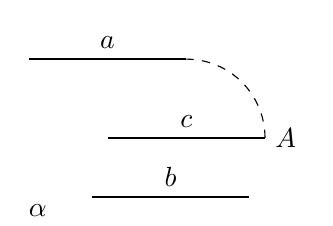
\begin{tikzpicture}[]
\tkzDefPoints{0/0/A, 3/0/B, 4/1.5/C, 1/1.5/D}
\tkzDrawPolygon[](A,B,C,D)
\draw[thick](.8,.25)--node[above]{$b$}(2.8,.25);
\draw[thick](1,1)--node[above]{$c$}(3,1)node[right]{$A$};
\draw[dashed](3,1)arc (0:90:1);
\draw[thick](2,2)--node[above]{$a$}(0,2);
\tkzLabelAngle[pos=.4](B,A,D){$\alpha$}

\end{tikzpicture}
\captionof{figure}{}
\end{minipage}

这个定理告诉我们，要证明一条已知直线和一个平面平行，只要在这个平面内找出一条直线和已知直线平行.



\begin{example}
    空间四边形相邻两边中点的连线，平行于经过另外两边的平面.

已知：空间四边形$ABCD$中，$E$、$F$分别是$AB$、$AD$的中点（图1.29）．
\end{example}

\begin{analyze}
要证$EF\parallel$平面$BCD$，只要证明$EF$平行于平面$BCD$内的某一直线.

求证：$EF\parallel$平面$BCD$.
\end{analyze}

\noindent
\begin{minipage}{.45\textwidth}
\CTEXindent
\begin{proof}
连结$BD$.

$\because\quad AF=EB, \quad AF=FD$

$\therefore\quad EF\parallel BD$

又$\because\quad BD\subset$平面$BCD$，$EF\not\subset$平面$BCD$

$\therefore\quad EF\parallel $平面$BCD$
\end{proof}
\end{minipage}
\hfill
\begin{minipage}{.45\textwidth}
\centering
\begin{tikzpicture}[]
    \tkzDefPoints{0/0/A1, 3.5/0/B1, 4.5/1.5/C1, 1/1.5/D1}
    \tkzDrawPolygon[](A1,B1,C1,D1)
\tkzDefPoints{1/.5/B, 3/.5/C, 2.3/1/D, 2.5/2.8/A}
\tkzDrawPolygon[thick](A,B,C,D)
\tkzDefMidPoint(A,B)\tkzGetPoint{E}  
\tkzDefMidPoint(A,D)\tkzGetPoint{F}  
\tkzDrawSegments[thick](B,D E,F)
\tkzLabelPoints[left](B,E)
\tkzLabelPoints[right](F,D,C)
\tkzLabelPoints[above](A)



\end{tikzpicture}
\captionof{figure}{}
\end{minipage}


现在我们来研究当直线$a$和平面$\alpha$平行时具有哪些性质.

从定义出发考虑，如果$\alpha\parallel a$，则$\alpha$与$a$无公共点，即$\alpha$上的点都不在$a$内，$\alpha$内的任何直线都和$a$无公共点. 这样$\alpha$内的直线$b$和$a$只可能是异面直线，或者是平行直线. 那么直线$b$在什么条件下才与$a$平行呢？由于这时$a$和$b$已无公共点，只要$a$和$b$在一个平面内就可以了，我们来证明这一探索.

已知：$a\parallel \alpha$, $a\subset \beta$, $\alpha\cap \beta=b$（图1.30）,

求证：$a\parallel b$.

\begin{analyze}
    可证明$a$、$b$两直线符合平行线定义.
\end{analyze}

\begin{multicols}{2}
\begin{proof}
$\because\quad a\parallel \alpha$

$\therefore\quad a$与$\alpha$无公共点.

又$\because\quad b\subset \alpha$

$\therefore\quad a$和$b$无公共点.

而$a\subset\beta,\quad b\subset\beta$,

$\therefore\quad a\parallel b$.
\end{proof}    
\end{multicols}

这样，我们就得到\textbf{直线和平面平行的性质定理}：如果一条直线和一个平面平行，经过这条直线的平面和这个平面相交，那么这条直线就和交线平行.


\noindent
\begin{minipage}{.48\textwidth}
\centering
\begin{tikzpicture}[]
    \tkzDefPoints{0/0/A, 3.5/0/B, 4.5/1.5/C, 1/1.5/D}
\tkzDefMidPoint(A,D) \tkzGetPoint{F}
\tkzDefMidPoint(B,C) \tkzGetPoint{E}
\tkzDrawPolygon[](A,B,E,F)
\tkzDefPoints{0/2.5/G}
\tkzDefPointBy[translation = from A to G](B) \tkzGetPoint{H}
\tkzDrawPolygon[](G,H,E,F)
\tkzInterLL(A,D)(E,F) \tkzGetPoint{tmp1}
\tkzInterLL(C,D)(E,H) \tkzGetPoint{tmp2}
\tkzDrawSegments[dashed](tmp1,D D,tmp2)
\tkzDrawSegments[](tmp2,C C,E)
\tkzLabelAngle[pos=.4](B,A,D){$\alpha$}
\tkzLabelAngle[pos=.4](F,G,H){$\beta$}
\node at (2,0.5){$b$};
\draw[thick](1,2)--node[above]{$a$}(3,2);

\end{tikzpicture}
\captionof{figure}{}
\end{minipage}
\hfill
\begin{minipage}{.48\textwidth}
\centering
\begin{tikzpicture}[]
\tkzDefPoints{0/0/A, 1.5/.8/B, 3/0/C, 0/2.5/A'}
\foreach \x in {B,C}
{
    \tkzDefPointBy[translation = from A to A'](\x) \tkzGetPoint{\x'}
}  
\tkzDrawPolygon[](A,B,C,C',B',A')
\tkzDrawSegments[thick](B,B')
\tkzLabelAngle[pos=.4](B,A,A'){$\alpha$}
\tkzLabelAngle[pos=.4](C',C,B){$\beta$}
\draw[thick](.8,1)--node[left]{$a$}(.8,2.5);
\draw[thick](2.1,1)--node[right]{$b$}(2.1,2.5);
\node at (1.5,2.6)[right]{$c$};
\end{tikzpicture}
\captionof{figure}{}
\end{minipage}


\begin{example}
    已知$a\parallel b$，$a\subset\alpha$, $b\subset \beta$, $\alpha\cap \beta=c$（图1.31）．

求证：$a\parallel c$, $b\parallel c$.
\end{example}

\begin{multicols}{2}
\begin{proof}
    $\because\quad a\parallel b,\quad a\not\subset \beta,\quad b\subset \beta$

$\therefore\quad a\parallel \beta$

$\because\quad a\subset \alpha,\quad \alpha\cap \beta=c$

$\therefore\quad a\parallel c$，同理$b\parallel c$.
\end{proof}
\end{multicols}


\noindent
\begin{minipage}{.55\textwidth}
\begin{example}
有一块木料如图1.32，已知它的各面都是平的，棱$BC$平行于面$A'C'$. 要经过木料表面$A'B'C'D'$内的一点$P$和棱$BC$将木料锯开，应怎样画线？所画的线和面$AC$有什么关系？
\end{example}

\begin{analyze}
    所画的线应过$P$点，且和$BC$在同一平面内.
\end{analyze}
\end{minipage}
\hfill
\begin{minipage}{.43\textwidth}
\centering
\begin{tikzpicture}[]
\tkzDefPoints{0/0/A, 3/0/B, 1.25/1.25/D, 0/2/A', 3/1.5/B'}
\tkzDefPointBy[translation= from A to D](B) \tkzGetPoint{C}  
\tkzDefPointBy[translation= from  A to A'](D) \tkzGetPoint{D'}  
\tkzDefPointBy[translation=  from B to B'](C) \tkzGetPoint{C'}  
\tkzDrawPolygon[thick](A,B,C,C',D',A')
\tkzDrawSegments[thick](A',B' B',C' B,B')
\tkzDrawSegments[dashed](A,D D,C D,D')
\tkzLabelPoints[left](A,A',D,D')
\tkzLabelPoints[right](B,C',C,B')
\tkzDefPointWith[linear, K=.3](B',A')\tkzGetPoint{E}
\tkzDefPointWith[linear, K=.3](C',D')\tkzGetPoint{F}
\tkzDefPointWith[linear, K=.3](F,E)\tkzGetPoint{P}
\fill[pattern=north west lines](E)--(B)--(C)--(F)--cycle;
\tkzLabelPoints[above](F)
\tkzLabelPoints[below left](E)
\tkzLabelPoints[left](P)
\tkzDrawPoints(P)
\tkzDrawSegments(E,F B,E)
\tkzDrawSegments[dashed](C,F)


\end{tikzpicture}
\captionof{figure}{}
\end{minipage}



\begin{solution}
\begin{enumerate}[(1)]
    \item $\because\quad BC\parallel $面$A'C'$，面$BC'$经过$BC$和面$A'C'$交于$B'C'$

$\therefore\quad BC\parallel B'C'$

经过点$P$，在面$A'C'$上画线段$EF\parallel B'C'$，根据公理4, $EF\parallel BC$.

$\therefore\quad EF\subset$平面$BF$，$BC\subset$平面$BF$. 连结$BE$和$CF$，$BE$、$CF$和$EF$就是所要画的线.

\item $\because\quad EF\parallel BC$，根据判定定理，则$EF\parallel $面$AC$；$BE$、$CF$显然都和面$AC$相交.
\end{enumerate}
\end{solution}

\begin{thm}{问：}
    本例中，若$AD\parallel BC$，$BC\parallel $平面$A'C'$，那么$AD$和平面$BC'$、平面$BF$、平面$A'C'$都有怎样的位置关系，为什么？
\end{thm}

\subsection*{1.8 练习}
\begin{enumerate}
\item 判断下列命题是否正确（$a$、$b$表示直线，$\alpha$表示平面）？
\begin{enumerate}[(1)]
\item 若$a\parallel b$, $b\subset \alpha$，则$a\parallel \alpha$\hfill (\qquad)
\item 若$a\parallel \alpha$, $b\parallel \alpha$，则$a\parallel b$.\hfill (\qquad)
\item 若$a\parallel b$，$b$与$\alpha$相交，则$a$与$\alpha$相交.\hfill (\qquad)
\item 若$a\parallel \alpha$，则夹在$a$与$\alpha$间的平行线段相等.\hfill (\qquad)
\item 若$a\parallel \alpha$，则$\alpha$内有无数条直线与$a$平行.\hfill (\qquad)
\end{enumerate}

    \item 若$a$、$b$是异面直线，则过$c$有一个平面与$b$平行．
    \item 若$a\parallel \alpha$, $P\in\alpha$, $P\in b$, $b\parallel a$，则$b\subset \alpha$.
    \item 已知正方体$ABCD-A_1B_1C_1D_1$．
    求证：
\begin{enumerate}[(1)]
 \item $BC\parallel $面$A_1ADD_1$
\item $BC_1\parallel $面$A_1ADD_1$
\item $C_1D\parallel $平面$ACB_1$
\end{enumerate}
    
\noindent
\begin{minipage}{.45\textwidth}
\centering
\begin{tikzpicture}[]
\tkzDefPoints{0/0/A, 2/0/B, .71/.71/D, 0/2/A_1}
  \tkzDefPointBy[translation = from A to D](B)\tkzGetPoint{C}
\foreach \x in {B,C,D}
{
  \tkzDefPointBy[translation = from A to A_1](\x)\tkzGetPoint{\x_1}
}
\tkzDrawPolygon[thick](A_1,B_1,C_1,D_1)
\tkzDrawSegments[thick](A,A_1 B,B_1 C,C_1 A,B C,B)
\tkzDrawSegments[dashed](A,D C,D D,D_1)
\tkzLabelPoints[left](A,A_1,D,D_1)
\tkzLabelPoints[right](B,B_1,C,C_1)

\end{tikzpicture}
\captionof*{figure}{第4题}
\end{minipage}
\hfill
\begin{minipage}{.45\textwidth}
\centering
\begin{tikzpicture}[]
\tkzDefPoints{0/0/A, 3/0/C, 1.5/2/D, 2/-1/B}
\tkzDrawPolygon[thick](A,B,C,D)  
\tkzDefMidPoint(A,B) \tkzGetPoint{E}
\tkzDefMidPoint(C,B) \tkzGetPoint{F}
\tkzDefMidPoint(C,D) \tkzGetPoint{G}

\draw[pattern=north east lines](E)--(F)--(G)--cycle;
\tkzLabelPoints[left](A)
\tkzLabelPoints[right](G,C,F)
\tkzLabelPoints[below](B,E)
\tkzLabelPoints[above](D)
\tkzInterLL(A,C)(G,E) \tkzGetPoint{tmp1}
\tkzInterLL(A,C)(G,F) \tkzGetPoint{tmp2}
\tkzDrawSegments(tmp1,A tmp2,C)


\end{tikzpicture}
\captionof*{figure}{第5题}
\end{minipage}

\item 空间四边形$ABCD$中，$E,F,G$分别是$AB,BC,CD$的中点。

求证：过$E$，$F$，$G$三点的平面与$AD$相交，并平分线段$AD$．
\end{enumerate}

\section{直线和平面垂直的判定和性质}
在直线和平面的三种位置关系中，我们已经研究过直线在平面内和直线与平面平行两种情形，现在来研究直线和平面相交的情形.首先研究特殊情况：直线和平面垂直.

如果一条直线和一个平面内的任何一条直线都垂直，我们说\textbf{这条直线和这个平面互相垂直}，直线叫做\textbf{平面的垂线}，平面叫做\textbf{直线的垂面}. 平面的垂线和平面一定相交，交点叫做\textbf{垂足}.

可以证明：过一点有且只有一条直线和一个平面垂直；过一点有且只有一个平面和一条直线垂直.

画直线和水平平面垂直时，要把直线画成和表示平面的平行四边形的横边垂直，如图1.33中的$AB$．

直线$\ell$和平面$\alpha$互相垂直，记作$\ell\bot \alpha$.

\begin{thm}
 {直线和平面垂直的判定定理1} 如果一条直线和一个平面内的两条相交直线都垂直，那么这条直线垂直于这个平面.   
\end{thm}

已知：$m\subset\alpha$, $n\subset \alpha$, $m\cap n=O$, $\ell\bot m$, $\ell\bot n$.

求证：$\ell\bot \alpha$.


\begin{analyze}
    要证明$\ell\bot \alpha$，只能根据定义. 就是要证明对任意的$g\subset \alpha$, 都有$\ell\bot g$.
\end{analyze}

\begin{proof}
设$g$是$\alpha$内的任一直线.

先证明$\ell$、$g$都通过点$O$的情况（图1.34）．


\noindent
\begin{minipage}{.48\textwidth}
\centering
\begin{tikzpicture}[scale=1.5]
\tkzDefPoints{0/0/A1, 2.5/0/B1, 3/1/C1, .5/1/D1}
\tkzDrawPolygon[](A1,B1,C1,D1)
\tkzLabelAngle[pos=.4](B1,A1,D1){$\alpha$}
\tkzDefPoints{1.5/.5/B, 1.5/2/A}
\tkzDefPointWith[linear, K=1.7](A,B) \tkzGetPoint{C}
\tkzInterLL(A,C)(A1,B1) \tkzGetPoint{tmp}
\tkzDrawSegments[thick](A,B tmp,C)
\tkzLabelPoints[right](A,B)
\node at (1.5,1.3)[right]{$\ell$};
\end{tikzpicture}
\captionof{figure}{}
\end{minipage}
\hfill
\begin{minipage}{.48\textwidth}
\centering
\begin{tikzpicture}[scale=1.5]
\tkzDefPoints{-.25/0/A1, 2.5/0/B1, 3/1/C1, 0.25/1/D1}
\tkzDrawPolygon[](A1,B1,C1,D1)
\tkzLabelAngle[pos=.25](B1,A1,D1){$\alpha$}
\tkzDefPoints{1.5/.75/O, 1.5/1.8/A, 1.5/2/ell, 1.5/-.4/A', 1.5/-.6/A''}
\tkzDefPoints{.7/.25/B, 2.2/.5/C}
\tkzDefPointWith[linear, K=.3](C,B) \tkzGetPoint{D}
\tkzDrawLines[add=0 and .3](O,C O,B)
\tkzDrawLines[add=0 and .9](O,D)
\tkzDrawLines[add=.2 and .3](B,C)
\tkzDrawSegments[thick](A,C A,D A,B A,O)


\tkzInterLL(A1,B1)(A',B) \tkzGetPoint{tmp1}
\tkzInterLL(A1,B1)(A',C) \tkzGetPoint{tmp2}
\tkzInterLL(A1,B1)(A',D) \tkzGetPoint{tmp3}
\tkzInterLL(A1,B1)(A',O) \tkzGetPoint{tmp4}
\tkzDrawSegments[thick](A',tmp1 A',tmp2 A',tmp3 A',tmp4)
\tkzDrawSegments[dashed](B,tmp1 C,tmp2 D,tmp3 O,tmp4)
\tkzLabelPoints[right](A,A')
\tkzDrawSegments[thick](A,ell A',A'')

\tkzLabelPoints[above left](B)
\tkzLabelPoints[above right](C)
\tkzLabelPoints[left](O)
\tkzLabelPoints[below](D)

\draw(O)--node[above]{$n$}(C);
\draw(O)--node[above]{$m$}(B);
\draw(O)--node[left]{$g$}(D);
\node at (ell)[left]{$\ell$};


\end{tikzpicture}
\captionof{figure}{}
\end{minipage}


在直线$\ell$上点$O$的两侧分别取点$A$、$A'$，使$AO=A'O$. 那么直线$m$、$n$都是线段$AA'$的垂直平分线，为了证明$\ell\bot g$，我们证明直线$g$也是线段$AA'$的垂直平分线.

当$g$与$m$（或$n$）重合时，根据已知$\ell\bot m$（或$n$），可知$\ell\bot g$成立. 当$g$与$m$、$n$都不重合时，在平面$\alpha$内作一条直线$CB$，与直线$m$、$n$、$g$分别交于点$C$、$B$、$E$. 连结$AC$、$A'C$、$AB$、$A'B$. 则有
\[AC=A'C,\quad AB=A'B\]

$\therefore\quad \triangle ACD\cong \triangle A'CD$，得
\[\angle ACD= \angle A'CD,\qquad AD=A'D\]

$\therefore\quad g$是$AA'$的垂直平分线.

$\therefore \quad \ell\bot g$

如果直线$\ell$、$g$中有一条或两条不经过点$O$，那么可过点$O$引它们的平行直线，由于过点$O$的这样两条直线所成的角就是直线$\ell$与$g$所成的角，同理可证这两条直线垂直. 因而$\ell\bot g$.

综上所述可得：$\ell\bot \alpha$.
\end{proof}

\begin{thm}
 {判定定理2} 如果两条平行直线中的一条垂直于一个平面，那么另一条也垂直于同一个平面.   
\end{thm}

已知：$a\parallel b$，$a\bot\alpha$（图1.35）

求证：$b\bot \alpha$.

\begin{analyze}
可以依据判定定理1，只要证明$b$垂直于平面$\alpha$内两条相交直线；也可根据定义，只要证明直线$b$垂直于平面$\alpha$内的任一直线. 下面用第二种证法.
\end{analyze}

\begin{proof}
设$g$是$\alpha$内任一直线.

\noindent
\begin{minipage}{.55\textwidth}
\CTEXindent
    $\because\quad a\bot \alpha,\quad g\subset \alpha$

    $\therefore\quad a\bot g$
    
    $\because\quad b\parallel a$
    
    $\therefore\quad b\bot g$，而$g$是$\alpha$内任一直线.
    
    $\therefore\quad b\bot\alpha$
\end{minipage}
\hfill
\begin{minipage}{.43\textwidth}
\centering
\begin{tikzpicture}[]
\tkzDefPoints{0/0/A1, 3/0/B1, 4/1/C1, 1/1/D1}
\tkzDrawPolygon[](A1,B1,C1,D1)
\tkzLabelAngle[pos=.5](B1,A1,D1){$\alpha$}
\draw[thick](1.4,2)--node[right]{$a$}(1.4,.6);
\draw[thick](3,2)--node[right]{$b$}(3,.6);
\draw[thick](1.25,.2)--node[below]{$g$}(2.5,.75);
\end{tikzpicture}
\captionof{figure}{}
\end{minipage}
\end{proof}




\begin{example}
在正方体 $ABCD-A_1B_1C_1D_1$中，$E$、$F$分别是$CC_1$、$DD_1$的中点，求证：
\begin{multicols}{2}
\begin{enumerate}[(1)]
    \item $AA_1\bot $平面$ABCD$
    \item $EF\bot $平面$A_1ADD_1$（图1.36）．
\end{enumerate}
\end{multicols}
\end{example}


\noindent
\begin{minipage}{.53\textwidth}
    \begin{analyze}
        \begin{enumerate}[(1)]
            \item 只要证明$AA_1$和面$ABCD$内的两条相交直线垂直.
            \item 可用判定定理2证明.
        \end{enumerate}
        \end{analyze}
\end{minipage}
\hfill
\begin{minipage}{.45\textwidth}
\centering
\begin{tikzpicture}[]
    \tkzDefPoints{0/0/A, 2/0/B, .71/.71/D, 0/2/A_1}
    \tkzDefPointBy[translation = from A to D](B)\tkzGetPoint{C}
  \foreach \x in {B,C,D}
  {
    \tkzDefPointBy[translation = from A to A_1](\x)\tkzGetPoint{\x_1}
  }
  \tkzDrawPolygon[thick](A_1,B_1,C_1,D_1)
  \tkzDrawSegments[thick](A,A_1 B,B_1 C,C_1 A,B C,B)
  \tkzDrawSegments[dashed](A,D C,D D,D_1)
  \tkzLabelPoints[left](A,A_1,D,D_1)
  \tkzLabelPoints[right](B,B_1,C,C_1)
\tkzDefMidPoint(D,D_1) \tkzGetPoint{F}  
\tkzDefMidPoint(C,C_1) \tkzGetPoint{E}  
\tkzDrawSegments[dashed](E,F)
\tkzLabelPoints[below left](E)
\tkzLabelPoints[below right](F)

\end{tikzpicture}
\captionof{figure}{}
\end{minipage}



\begin{proof}
在正方体$ABCD-A_1B_1C_1D_1$中，
$A_1A\bot AB,\quad A_1A\bot AD,\quad AB\cap AD=A$

$\therefore\quad A_1A\bot $平面$ABCD$.

同理$CD\bot $平面$A_1ADD_1$，而$E$，$F$分别是$CC_1$和$DD_1$的中点，


\noindent
\begin{minipage}{.45\textwidth}\CTEXindent
$\therefore\quad CE=DF$.

又$CE\parallel DF$

$\therefore\quad CEFD$为平行四边形

$\therefore\quad EF\parallel CD$.

$\because\quad CD\bot $平面$A_1ADD_1$

$\therefore\quad EF\bot $平面$A_1ADD_1$．
\end{minipage}
\hfill
\begin{minipage}{.45\textwidth}
\centering
\begin{tikzpicture}[]
    \tkzDefPoints{0/0/A, 2/0/B, .71/.71/D, 0/2/A_1}
    \tkzDefPointBy[translation = from A to D](B)\tkzGetPoint{C}
  \foreach \x in {B,C,D}
  {
    \tkzDefPointBy[translation = from A to A_1](\x)\tkzGetPoint{\x_1}
  }
  \tkzDrawPolygon[thick](A_1,B_1,C_1,D_1)
  \tkzDrawSegments[thick](A,A_1 B,B_1 C,C_1 A,B C,B)
  \tkzDrawSegments[dashed](A,D C,D D,D_1)
\draw[thick](B)--node[above right]{$c$}(A_1);
\draw(A_1)--node[left]{$a$}(D_1);
\draw(B_1)--node[right]{$b$}(C_1);
\node at (1.3,2.4){$M$};
\end{tikzpicture}
\captionof{figure}{}
\end{minipage}
\end{proof}
 
\begin{remark}
应用判定定理1证明直线和平面垂直时，注意定理条件“一条直线和一个平面内的两条相交直线都垂直”中的“相交”二字. 如果去掉这两个字，命题就不成立，如图1.37，$a\subset M$, $b\subset M$, $a\parallel b$, $c\bot a$, $c\bot b$. 但$c$不垂直于$M$. 所以不能认为一直线垂直于一平面内的两条直线，这直线就和这平面垂直.
\end{remark}


\begin{example}
    空间四边形$ABCD$中，连结$AC$、$BD$，若$AB=AC$, $BD=DC$. 求证：$AD\bot BC$.
\end{example}

\begin{analyze}
由直线和平面垂直的定义知道，要证两直线垂直，可以证明一条直线和另一直线所在的一个平面垂直.

本题中，$\because\quad AB=AC$

$\therefore\quad $若$E$是$BC$的中点可得$AE\bot BC$. 

同理，$\because\quad DB=DC$，则$DE\bot BC$.

根据判定定理1，易证$BC\bot $平面$ADE$．$AD\subset $平面$ADE$，即可证出$BC\bot AD$.
\end{analyze}

\begin{proof}
取$BC$的中点$E$，连结$AE$、$DE$（图1.38）．

\noindent
\begin{minipage}{.45\textwidth}\CTEXindent
$\because\quad AB=AC$

$\therefore\quad BC\bot AE$

$\because\quad DB=DC$

$\therefore\quad BC\bot DE$.

又 $AE\cap DE=E$

$\therefore\quad BC\bot $平面$ADE$.

$\because\quad AD\subset$平面$ADE$，

$\therefore\quad BC\bot AD$

\end{minipage}
\hfill
\begin{minipage}{.45\textwidth}
\centering
\begin{tikzpicture}[]
\tkzDefPoints{0/0/B, 4/0/C, 2/0/E, 1.5/1/D, 2/3/A}
\tkzDrawPolygon[](A,B,C)  
\tkzDrawPolygon[](D,B,C)  
\draw[pattern=north east lines](A)--(D)--(E)--cycle;
\tkzLabelPoints[below](B,C,E,D)
\tkzLabelPoints[above](A)
\end{tikzpicture}
\captionof{figure}{}
\end{minipage}

\end{proof}

下面研究直线和平面垂直的性质.

由直线$a$和平面$\alpha$垂直，可以得出什么结果呢？根据直线和平面垂直的定义可得到这直线$a$和平面$\alpha$内的任一直线都垂直. 若直线$a$和直线$b$都垂直于$\alpha$，那么直线$a$和$b$有什么位置关系呢？（图1.39）

\noindent
\begin{minipage}{.45\textwidth}
\centering
\begin{tikzpicture}[]
    \tkzDefPoints{0/0/A1, 3/0/B1, 4/1/C1, 1/1/D1}
    \tkzDrawPolygon[](A1,B1,C1,D1)
    \tkzLabelAngle[pos=.5](B1,A1,D1){$\alpha$}
    \draw[thick](1.4,2)--node[right]{$a$}(1.4,.6);
    \draw[thick](3,2)--node[right]{$b$}(3,.6);

    \end{tikzpicture}
    \captionof{figure}{}
\end{minipage}
\hfill
\begin{minipage}{.45\textwidth}
\centering
\begin{tikzpicture}[]
\tkzDefPoints{0/0/A1, 3/0/B1, 4/1/C1, 1/1/D1}
\tkzDrawPolygon[](A1,B1,C1,D1)
\tkzLabelAngle[pos=.5](B1,A1,D1){$\alpha$}
\draw[thick](1.4,2)--node[left]{$a$}(1.4,.6);
\draw[thick](3,2)--node[right]{$(b')$}(3,.6)node[below]{$O$};
\node at (3,1.3)[left]{$b$};
\end{tikzpicture}
\captionof{figure}{}
\end{minipage}

由观察得到启发，它们可能平行. 能证明吗？我们试一试.

已知：直线$a\bot$平面$\alpha$，直线$b\bot$平面$\alpha$（图1.40）．

求证：$a\parallel b$.

\begin{proof}
    设$b\cap \alpha=O$，过$O$作直线$b'$，使$b'\parallel a$.

$\because\quad    a\bot \alpha$

$\therefore\quad b'\bot \alpha$（判定定理2）．

经过同一点$O$只有一条直线与平面$\alpha$垂直\footnote{可证明：若$D\in b$, $O\in b'$，$b'\bot\alpha$, $b\bot\alpha$，则$b$与$b'$重合；若$b$与$b''$相交，则确定一平面$\beta$，设$\beta\cap \alpha=C$.

$\because\quad b\bot\alpha\qquad \therefore\quad b\bot c$. 同理$b'\bot c$

而$b\cap b'=O$，且与$c$都在$\beta$内，这是不可能的

$\therefore\quad b$与$b'$重合.}. 所以$b'$和$b$是同一直线

$\because\quad b'\parallel a$

$\therefore\quad b\parallel a$.
\end{proof}

于是我们得到：

\begin{thm}
{直线和平面垂直的性质定理}
如果两条直线同垂直于一个平面，那么这两条直线平行.    
\end{thm}

类比平面几何中点到直线的距离的概念，我们可以定义点到平面的距离.

\begin{thm}
    {定义} 从平面外一点向这个平面引垂线，这个点和垂足间的距离叫做这个\textbf{点到这个平面的距离}.
\end{thm}

\begin{example}
    如果一条直线和一个平面平行，那么这条直线上的各点到这个平面的距离都相等.

已知：直线$\ell\parallel $平面$\alpha$.

求证：$\ell$上各点到$\alpha$上的距离相等（图1.41）．
\end{example}

\begin{analyze}
只需在这条直线上任取两点，证明它们到这个平面的距离相等即可. 这只要把问题转化到一个平面上，再利用平面图形的性质来解决.
\end{analyze}

\noindent
\begin{minipage}{.58\textwidth}\CTEXindent
\begin{proof}
过直线$\ell$上任意两点$A$、$B$分别引平面$\alpha$的垂线$AA'$、$BB'$，垂足分别为$A'$、$B'$.

$\because\quad AA'\bot \alpha,\quad BB'\bot\alpha$

$\therefore\quad AA'\parallel BB'$

设经过直线$AA'$和$BB'$的平面为$\beta$， $\beta\cap \alpha=A'B'$

$\because\quad \ell\parallel \alpha$

$\therefore\quad \ell\parallel A'B'$

$\therefore\quad AA'=BB'$，
即直线$\ell$上各点到平面的距离相等.
\end{proof}
\end{minipage}
\hfill
\begin{minipage}{.4\textwidth}
\centering
\begin{tikzpicture}[]
\tkzDefPoints{0/0/A1, 3/0/B1, 4/1/B2, 1/1/A2, 1/3/A3, 4/3/B3, 4.5/1.5/B4}
\tkzDefPointBy[translation = from B1 to B4](A1) \tkzGetPoint{A4}
\tkzDrawPolygon(A1,B1,B2,A2)
\tkzDrawPolygon(A2,B2,B3,A3)
\tkzInterLL(B2,B3)(A4,B4)  \tkzGetPoint{tmp}
\tkzDrawSegments[dashed](A2,A4 A4,tmp)
\tkzDrawSegments[](B4,B2 B4,tmp)
\tkzLabelAngle[pos=.4](B1,A1,A2){$\alpha$}
\tkzLabelAngle[pos=.4](A2,A3,B3){$\beta$}

\draw(2,1)node[below]{$A'$}--(2,2.25)node[above]{$A$};
\draw(3.5,1)node[below]{$B'$}--(3.5,2.25)node[above]{$B$};
\draw[thick](1.75,2.25)--node[above]{$\ell$}(3.75,2.25);
\end{tikzpicture}
\captionof{figure}{}
\end{minipage}

这个例题为我们定义直线到平面的距离提供了依据. 于是，我们有：

\begin{thm}
    {定义} 一条直线和一个平面平行，这条直线上任意一点到这个平面的距离叫做\textbf{这条直线到这个平面的距离}.
\end{thm}

\subsection*{1.9 练习}
\begin{enumerate}
    \item 判断题：
\begin{enumerate}[(1)]
\item 一直线和一个平面内无数条直线垂直，则这直线和这平面垂直.\hfill(\quad )
\item 一直线垂直于一个三角形的两个边，则它必垂直于第三边.\hfill(\quad )
\item 三条直线$a$、$b$、$c$共点，且两两垂直，则每一直线垂直于另两条直线所确定的平面.\hfill(\quad )
\item 一条直线上有两点到一个平面的距离相等，则这直线和这平面平行. (\quad )
\item 两条异面直线不能同时垂直于一个平面．\hfill(\quad )
\end{enumerate}

\item 安装日光灯时，怎样才能使灯管和天棚、地板平行？
\item 已知$AB\cap\alpha=O$，$AB\bot\alpha$, 且$AO=BO$.

求证：对任意的$P\in\alpha$，有$PA=PB$.
\item 已知：$\triangle ABC$在平面$\alpha$内，$SB\bot\alpha$, $\angle BAC=30^{\circ}$, $SB=5$，$AB=8$，求点$S$到直线$AC$的距离.
\item 矩形$ABEF$和矩形$EFCD$不共面，已知$EF=4$，$AD=5$，求平行直线$AB$和$CD$之间的距离．
\item 空间四边形$ABCD$中，$AB=BC$, $CD=DA$, 点$M$、$N$、$P$、$Q$分别是$AB$、$BC$、$CD$、$DA$的中点. 求证：四边形$MNPQ$是矩形.
\item 已知$a\parallel \alpha$，$b\bot\alpha$，求证：$a\bot b$.
\item 已知平面$\alpha\cap$平面$\beta=CD$, $PA\bot\alpha$于$A$，$PB\bot\beta$于$B$. 求证：$CD\bot AB$.

\end{enumerate}

\section{直线在平面上的射影 直线和平面所成的角}
\begin{thm}
{定义} 自一点向一平面引垂线，垂足叫做这个\textbf{点在平面上的射影}. 这个点与垂足间的线段叫做这个\textbf{点到这个面的垂线段}.
\end{thm}

显然，当点$P\in$平面$\alpha$时，$P$在$\alpha$上的射影就是点$P$自身.

\begin{thm}
{定义} 一个图形$F$上的所有点在平面$\alpha$上的射影的集合$F'$，叫做\textbf{图形$F$在平面$\alpha$上的射影}（图1.42）．
\end{thm}

\begin{figure}[thp]
    \centering
\begin{tikzpicture}
\tkzDefPoints{-2/0/a, 4/0/b, 5.5/2/c, -.5/2/d}
\tkzDrawPolygon(a,b,c,d)
\tkzLabelAngle[pos=.4](b,a,d){$\alpha$}
\draw[thick](0,4)node[left]{$A$}--(0,3)node[left]{$B$};
\draw[dashed](0,3)--(0,1.3)node[below]{$A'(B')$};
\draw[thick](1,3.2)node[above]{$A$}--node[above]{$\ell$}(2,3.5)node[above]{$B$};
\draw[thick](1,1.5)node[below]{$A'$}--node[above]{$\ell'$}(2,1.5)node[below]{$B'$};
\draw[dashed](1,3.2)--(1,1.5);
\draw[dashed](2,3.5)--(2,1.5);

\draw[thick](3,4)node[above]{$A$}--(4,4)node[above]{$B$}--(3.2,3.4)node[below right]{$C$}--cycle;

\draw[thick](3,1.6)node[left]{$A'$}--(4,1.6)node[right]{$B'$}--(3.2,1.2)node[below]{$C'$}--cycle;

\draw[dashed](3,4)--(3,1.6);
\draw[dashed](4,4)--(4,1.6);
\draw[dashed](3.2,3.4)--(3.2,1.2);


\end{tikzpicture}
    \caption{}
\end{figure}

\begin{thm}
{定义} 一条直线和一个平面相交，但不和这个平面垂直，这条直线叫做\textbf{这个平面的斜线}，斜线和平面的交点叫做\textbf{斜足}，斜线上一点与斜足间的线段叫做\textbf{这点到这个平面的斜线段}.    
\end{thm}

由图形$F$在平面$\alpha$上的射影的定义易知：平面$\alpha$的垂线在平面$\alpha$上的射影是一个点，平面$\alpha$的斜线在$\alpha$上的射影是一条直线.

\begin{thm}
 {定义} 过斜线上斜足以外的一点向平面引垂线，过垂足和斜足的直线是\textbf{斜线在这个平面上的射影}，垂足与斜足间的线段是这点到平面的\textbf{斜线段在这个平面上的射影}. 斜线上任意一点在平面上的射影，一定在斜线的射影上.   
\end{thm}

\noindent
\begin{minipage}{.63\textwidth}\CTEXindent

    如图1.43对于平面$\alpha$，直线$AB$是垂线，垂足$B$是点$A$的射影，也是垂线$AB$的射影；直线$AC$是斜线，$C$是斜足，直线$BC$是斜线$AC$的射影；线段$AB$是垂线段，线段$AC$是斜线段，线段$BC$是斜线段$AC$的射影.

    根据直角三角形性质，我们很容易得到：
\end{minipage}
\hfill
\begin{minipage}{.35\textwidth}
\centering
\begin{tikzpicture}[]
    \tkzDefPoints{0/0/a, 3/0/b, 4/1.5/c, 1/1.5/d}
    \tkzDrawPolygon(a,b,c,d)
    \tkzLabelAngle[pos=.4](b,a,d){$\alpha$}
    \tkzDefPoints{1.5/.5/B, 2.5/.5/C, 1.5/2/A}
    \tkzDrawLines[add=.6 and .3, thick](B,C)
    \tkzDrawLines[add=.2 and 0, thick](A,C A,B)
    \tkzLabelPoints[right](A)
    \tkzLabelPoints[above right](C)
    \tkzLabelPoints[above left](B)
    \draw[thick](1.5,0)--(1.5,-.5);
    \tkzDefPointWith[linear, K=1.6](A,C) \tkzGetPoint{D}
    \tkzInterLL(A,D)(a,b) \tkzGetPoint{tmp}
    \draw[thick](tmp)--(D);
\end{tikzpicture}
\captionof{figure}{}
\end{minipage}




\begin{thm}
{定理} 从平面外一点向这个平面所引的垂线段和斜线段中，
\begin{enumerate}[(1)]
\item 射影相等的两条斜线段相等，射影较长的斜线段也较长；
\item 相等的斜线段的射影相等，较长的斜线段的射影也较长；
\item 垂线段比任何一条斜线段都短．    
\end{enumerate}
\end{thm}

已知：$AO$是平面$\alpha$的垂线段，$AB$、$AC$是平面$\alpha$的斜线段（图1.44）．

\noindent
\begin{minipage}{.6\textwidth}
    求证：
    \begin{enumerate}[(1)]
        \item $OB=OC\quad\Rightarrow\quad AB=AC$
    
        $OB>OC\quad\Rightarrow\quad AB>AC$
        \item $AB=AC\quad\Rightarrow\quad OB=OC$
    
        $AB>AC\quad\Rightarrow\quad OB>OC$
    \item 对任意的$B\in\alpha$，当$B$不与$O$重合时，有$AB>AO$
    \end{enumerate}
\end{minipage}
\hfill
\begin{minipage}{.38\textwidth}
\centering
\begin{tikzpicture}[]
    \tkzDefPoints{0/0/a, 3/0/b, 4/1.5/c, 1/1.5/d}
    \tkzDrawPolygon(a,b,c,d)
    \tkzLabelAngle[pos=.4](b,a,d){$\alpha$}
    \tkzDefPoints{1/.5/B, 2.2/1/O, 3/.7/C, 2.2/3/A}
    \tkzDrawPolygon[thick](A,B,O,C)
    \tkzDrawSegments[thick](A,O)
    \tkzLabelPoints[above](A)
    \tkzLabelPoints[right](C)
    \tkzLabelPoints[left](B)
    \tkzLabelPoints[below](O)
\end{tikzpicture}
\captionof{figure}{}
\end{minipage}

\begin{proof}
    （由读者自己完成.）
\end{proof}

现在我们来研究直线和平面所成的角的问题.

\begin{thm}
  {定理} 平面的斜线和平面内经过斜足的所有直线所成的一切角中，以斜线和它在平面上的射影所成的角最小.  
\end{thm}

已知：$\ell$是平面$\alpha$的斜线，$O$为斜足，$A\in\ell$, $A$在$\alpha$上的射影是$B$，$OD$为$\alpha$内过$O$点的任一直线（图1.45）.

求证：$\angle AOB<\angle AOD$.

\noindent
\begin{minipage}{.58\textwidth}\CTEXindent
\begin{proof}
    设$AC\bot OD$于$C$，
    
$\because\quad AB$为垂线段，$AC$为$\alpha$的斜线段.

$\therefore\quad AB<AC$\\
又$\sin\angle AOB=\frac{AB}{AO},\quad \sin\angle AOC=\frac{AC}{AO}$

$\therefore\quad \sin\angle AOB< \sin\angle AOC$

而$\angle AOB$, $\angle AOC$都是锐角，

$\therefore\quad \angle AOB<\angle AOC$
\end{proof}
\end{minipage}
\hfill
\begin{minipage}{.4\textwidth}
\centering
\begin{tikzpicture}[]
    \tkzDefPoints{-1/0/a, 3/0/b, 4/1.5/c, 0/1.5/d}
    \tkzDrawPolygon(a,b,c,d)
    \tkzLabelAngle[pos=.4](b,a,d){$\alpha$}
    \tkzDefPoints{1/1/O, 2.5/1/B, 2/.55/C, 2.5/2.5/A}
    \tkzDrawSegments[thick](A,B A,C)
    \tkzLabelPoints[above](A,O)
    \tkzLabelPoints[below](B,C)
    \tkzDrawLines[add=.3 and .3, thick](O,B)
    \tkzDrawLines[add=.4 and 0, thick](A,O C,O)
    \node at (3.2,1){$\ell'$};
    \node at (2.5,.3){$D$};
    \tkzMarkAngles[size=.5, mark=none](B,O,A)
    \tkzLabelAngle[pos=.7](B,O,A){$\theta$}
    \tkzDefPointWith[linear, K=2](A,O)  \tkzGetPoint{A'}
    \tkzInterLL(A,O)(a,b)\tkzGetPoint{tmp}
    \draw[dashed](tmp)--(O);
    \draw[thick](tmp)--(A');
\end{tikzpicture}
\captionof{figure}{}
\end{minipage}

\begin{thm}
    {定义} 平面的一条斜线和它在平面上的射影所成的锐角，叫做这条\textbf{斜线和这个平面所成的角}.
\end{thm}

若直线和平面垂直，我们就说这条直线和这个平面所成的角是直角. 若一条直线和一个平面平行或在平面内，我们
说这条直线和这个平面所成的角是$0^{\circ}$的角．



\noindent
\begin{minipage}{.55\textwidth}\CTEXindent
    \begin{example}
        直线$\ell$和平面$\alpha$所成的角是$\theta$，$\ell$上的线段$AB$在$\alpha$上的射影是线段$A'B'$（图1.46）．则
    \[A'B'=AB\cdot \cos\theta\]
    \end{example}
    
    \begin{proof}
    $\because\quad AA'\bot\alpha,\quad BB'\bot \alpha$,
    
    $\therefore\quad AA'\parallel BB'$
    
    设$AA'$和$BB'$确定的平面为$\beta$（图1.46). 过$A$作$AB''\parallel  A'B'$交$BB'$于$B''$, 则$\angle BAB''=\theta$, 且$AA'BB'$是矩形.
    
    $\therefore\quad A'B'=AB''=AB\cos\theta$.
    \end{proof}
\end{minipage}
\hfill
\begin{minipage}{.43\textwidth}
\centering
\begin{tikzpicture}[]
    \tkzDefPoints{-1/0/a, 3/0/b, 4/1.5/c, 0/1.5/d}
    \tkzDrawPolygon(a,b,c,d)
    \tkzLabelAngle[pos=.4](b,a,d){$\alpha$}
    \tkzDefPoints{0/.5/O, 2.5/.5/B', 2.5/3/B}
    \tkzDefPointWith[linear, K=0.6](O,B) \tkzGetPoint{A}
    \tkzDefPointWith[linear, K=0.6](O,B') \tkzGetPoint{A'}
    \tkzDefPointWith[linear, K=0.6](B',B) \tkzGetPoint{B''}
    \tkzDrawSegments[thick](A,B'' O,B' A,A' B,B') 
    \tkzDrawLines[add= 0 and .2, thick](O,B) 
    \tkzLabelPoints[below](A',B')
    \tkzLabelPoints[right](B'')
    \tkzLabelPoints[left](A,B)
    \tkzLabelAngles[pos=.6](B'',A,B B',O,B){$\theta$} 
    \tkzMarkAngles[mark=none, size=.4](B'',A,B B',O,B) 
    \node at (3.1,3.5){$\ell$};
\end{tikzpicture}
\captionof{figure}{}
\end{minipage}


\subsection*{1.10 练习}
\begin{enumerate}
    \item 判断题：
\begin{enumerate}[(1)]
\item 在一平面内的射影为直线的图形只能是直线。\hfill(\quad)
\item 若两条斜线段在同一平面上的射影长相等，则这两
条斜线段的长也相等.\hfill(\quad)
\item 若平面$\alpha$的两条斜线与$\alpha$成的角相等，则过两直线平行.\hfill(\quad)
\item 与$\triangle ABC$的三个顶点距离相等的点，一定在过三角形的外心且与$\triangle ABC$所在平面垂直的直线上.\hfill(\quad)
\item 若$P$点与$\triangle ABC$三顶点的连线与$\triangle ABC$所在平面成的角相等，则$P$在$\triangle ABC$所在平面的射影是$\triangle ABC$的外心.\hfill(\quad)
\end{enumerate}

\item 在正方体$ABCD-A_1B_1C_1D_1$中，求
\begin{enumerate}[(1)]
    \item $A_1C_1$与正方体各面成的角的大小，
    \item $D_1B$与面$A_1ADD_1$所成角的正切值.
\end{enumerate}

\begin{minipage}{.48\textwidth}
    \centering
    \begin{tikzpicture}[]
\tkzDefPoints{0/0/A, 2/0/B, 2.71/.71/C, .71/.71/D, 0/2/A_1}
\foreach \x in {B,C,D}
{
   \tkzDefPointBy[translation = from A to A_1](\x) \tkzGetPoint{\x_1}
}
\tkzDrawPolygon[thick](A,B,C,C_1,D_1,A_1)
\tkzDrawSegments[thick](A_1,B_1 B_1,C_1 A_1,C_1 B,B_1) 
\tkzDrawSegments[dashed](B,D_1 A,D C,D D,D_1) 
\tkzLabelPoints[left](A,A_1,D,D_1)
\tkzLabelPoints[right](B,B_1,C,C_1)
    \end{tikzpicture}
    \captionof*{figure}{第2题}
\end{minipage}\hfill
\begin{minipage}{.48\textwidth}
    \centering
    \begin{tikzpicture}[]
\tkzDefPoints{-.5/0/a, 3/0/b, 4/1.5/c, 0.5/1.5/d}
\tkzDrawPolygon(a,b,c,d)
\tkzLabelAngle[pos=.4](b,a,d){$\alpha$}
\tkzDefPoints{1/1/A, 3/1/D, 3/3/P, 2/.4/B}
\tkzDrawPolygon[thick](A,P,D)
\tkzDrawSegments[thick](P,B D,B)
\tkzLabelPoints[left](A,B)
\tkzLabelPoints[right](D)
\tkzLabelPoints[above](P)
    \end{tikzpicture}
    \captionof*{figure}{第3题}
\end{minipage}


\item 已知：$PD\bot $平面$\alpha$，$A\in\alpha$, $B\in\alpha$, $\angle APB=60^{\circ}$, $PA$, $PB$与$\alpha$成的角分别是$30^{\circ}$和$45^{\circ}$，求$\angle ADB$的余弦值.
\end{enumerate}
